\documentclass{beamer}

%\mode<presentation>
%{
 %\usetheme[navigation=true]{DERI}
 %\setbeamercovered{transparent}
 %\beamertemplateballitem
%}
%\usepackage{beamerthemeDERI}

\usepackage{beamerthemeinsight/insight}
\setbeamercovered{transparent}

\usepackage[medium]{ubuntu}

% Make the text wider on a frame
\newcommand\Wider[2][3em]{%
\makebox[\linewidth][c]{%
  \begin{minipage}{\dimexpr\textwidth+#1\relax}
  \raggedright#2
  \end{minipage}%
  }%
}

% Switch implementation
\usepackage{xifthen}
\newcommand{\ifequals}[3]{\ifthenelse{\equal{#1}{#2}}{#3}{}}
\newcommand{\case}[2]{#1 #2} % Dummy, so \renewcommand has something to overwrite...
\newenvironment{switch}[1]{\renewcommand{\case}{\ifequals{#1}}}{}

\usepackage{url}

\usepackage{minted}

\usepackage{multicol}

\usepackage{graphicx}
\usepackage{caption}
\usepackage{subcaption}

\usepackage[french]{babel}

\usepackage{tikz}
\usetikzlibrary{patterns,shapes,arrows,positioning,shapes.geometric,calc,arrows.meta,fadings,decorations.markings,decorations.shapes}

\tikzset{red highlight node/.style={fill=red!24}}
\tikzset{green highlight node/.style={fill=green!24}}
\tikzset{red highlight edge/.style={draw,line width=5pt,-,red!50}}
\tikzset{green highlight edge/.style={draw,line width=5pt,-,green!50}}

\usepackage{pgfplots}
\pgfplotsset{compat=1.10}

% Matrix
\usepackage{pgfplotstable}
\newcommand{\Size}{1cm}% Adjust size of square as desired
\tikzset{Square/.style={
        inner sep=0pt,
        text width=\Size, 
        minimum size=\Size,
        draw=black,
        fill=white,
        align=center
    }
}
\tikzset{Red Square/.style={
        inner sep=0pt,
        text width=\Size, 
        minimum size=\Size,
        draw=black,
        fill=red,
        align=center
    }
}
\tikzset{Blue Square/.style={
        inner sep=0pt,
        text width=\Size, 
        minimum size=\Size,
        draw=black,
        fill=blue,
        align=center
    }
}
\tikzset{Orange Square/.style={
        inner sep=0pt,
        text width=\Size, 
        minimum size=\Size,
        draw=black,
        fill=orange,
        align=center
    }
}
\tikzset{Green Square/.style={
        inner sep=0pt,
        text width=\Size, 
        minimum size=\Size,
        draw=black,
        fill=black!30!green,
        align=center
    }
}
\tikzset{Black Square/.style={
        inner sep=0pt,
        text width=\Size, 
        minimum size=\Size,
        draw=black,
        fill=black,
        align=center
    }
}
\tikzset{Magenta Square/.style={
        inner sep=0pt,
        text width=\Size, 
        minimum size=\Size,
        draw=black,
        fill=magenta,
        align=center
    }
}
\tikzset{Brown Square/.style={
        inner sep=0pt,
        text width=\Size, 
        minimum size=\Size,
        draw=black,
        fill=brown,
        align=center
    }
}
\tikzset{Magenta Brown Square/.style={
        inner sep=0pt,
        text width=\Size, 
        minimum size=\Size,
        draw=black,
        fill=brown,
        align=center,
        postaction={
            pattern=north west lines,
            pattern color=magenta
        }
    }
}

%%%
%%% DIM COLORS
%%%

\tikzset{Dim Red Square/.style={
        inner sep=0pt,
        text width=\Size, 
        minimum size=\Size,
        draw=black,
        fill=red!50,
        align=center
    }
}
\tikzset{Dim Blue Square/.style={
        inner sep=0pt,
        text width=\Size, 
        minimum size=\Size,
        draw=black,
        fill=blue!50,
        align=center
    }
}
\tikzset{Dim Orange Square/.style={
        inner sep=0pt,
        text width=\Size, 
        minimum size=\Size,
        draw=black,
        fill=orange!50,
        align=center
    }
}
\tikzset{Dim Green Square/.style={
        inner sep=0pt,
        text width=\Size, 
        minimum size=\Size,
        draw=black,
        fill=black!30!green!50,
        align=center
    }
}
\tikzset{Dim Black Square/.style={
        inner sep=0pt,
        text width=\Size, 
        minimum size=\Size,
        draw=black,
        fill=black!50,
        align=center
    }
}
\tikzset{Dim Magenta Square/.style={
        inner sep=0pt,
        text width=\Size, 
        minimum size=\Size,
        draw=black,
        fill=magenta!50,
        align=center
    }
}
\tikzset{Dim Brown Square/.style={
        inner sep=0pt,
        text width=\Size, 
        minimum size=\Size,
        draw=black,
        fill=brown!50,
        align=center
    }
}
\tikzset{Dim Magenta Brown Square/.style={
        inner sep=0pt,
        text width=\Size, 
        minimum size=\Size,
        draw=black,
        fill=brown!50,
        align=center,
        postaction={
            pattern=north west lines,
            pattern color=magenta!50
        }
    }
}

\title{Making Sense of Web Data}
\author{St\'ephane Campinas}
\institute{
    Insight Centre for Data Analytics\\
    National University of Ireland, Galway
}
\date{Thesis VIVA, 13 December 2016}

\begin{document}

\frame{\titlepage}

\frame{
    \frametitle{Table of Contents}
    \begin{multicols}{2}
        \tableofcontents
    \end{multicols}
}

\section{Introduction}

\subsection{Motivation}

\frame{
    \frametitle{Evolution of Web Data}
    \begin{figure}
        \centering
        \begin{subfigure}{.2\textwidth}
            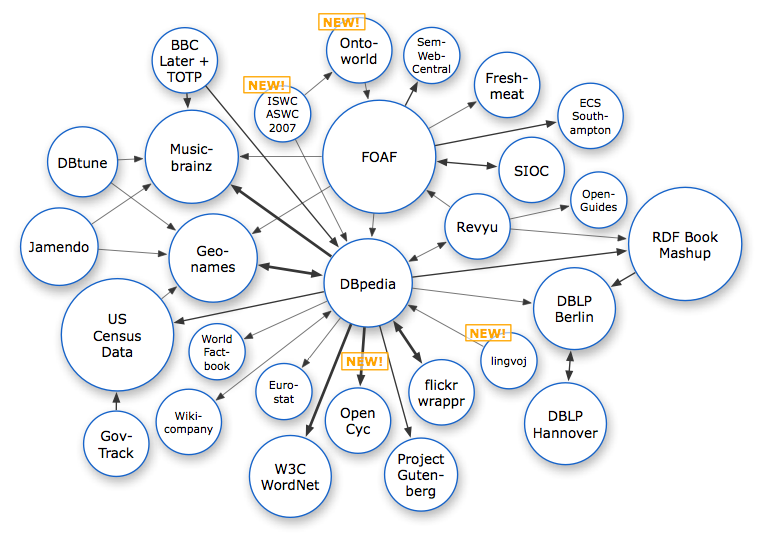
\includegraphics[width=\textwidth]{images/introduction/lod-cloud-2007-11-07}
        \end{subfigure}
        \begin{subfigure}{.215\textwidth}
            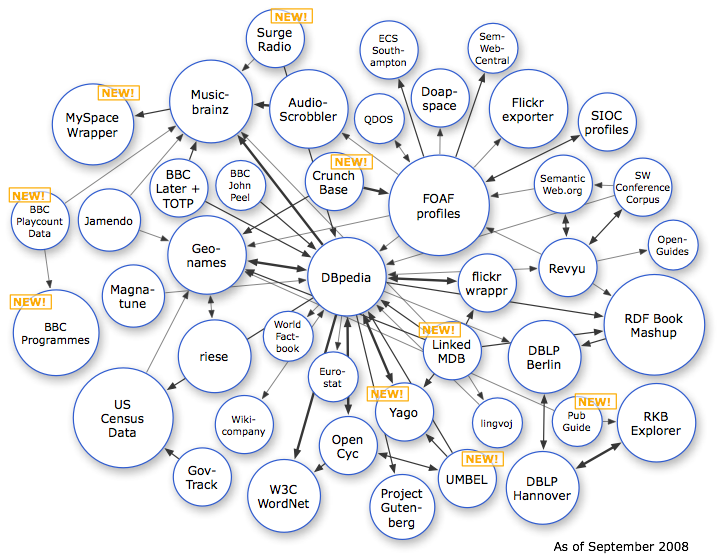
\includegraphics[width=\textwidth]{images/introduction/lod-cloud-2008-09-18}
        \end{subfigure}
        \begin{subfigure}{.225\textwidth}
            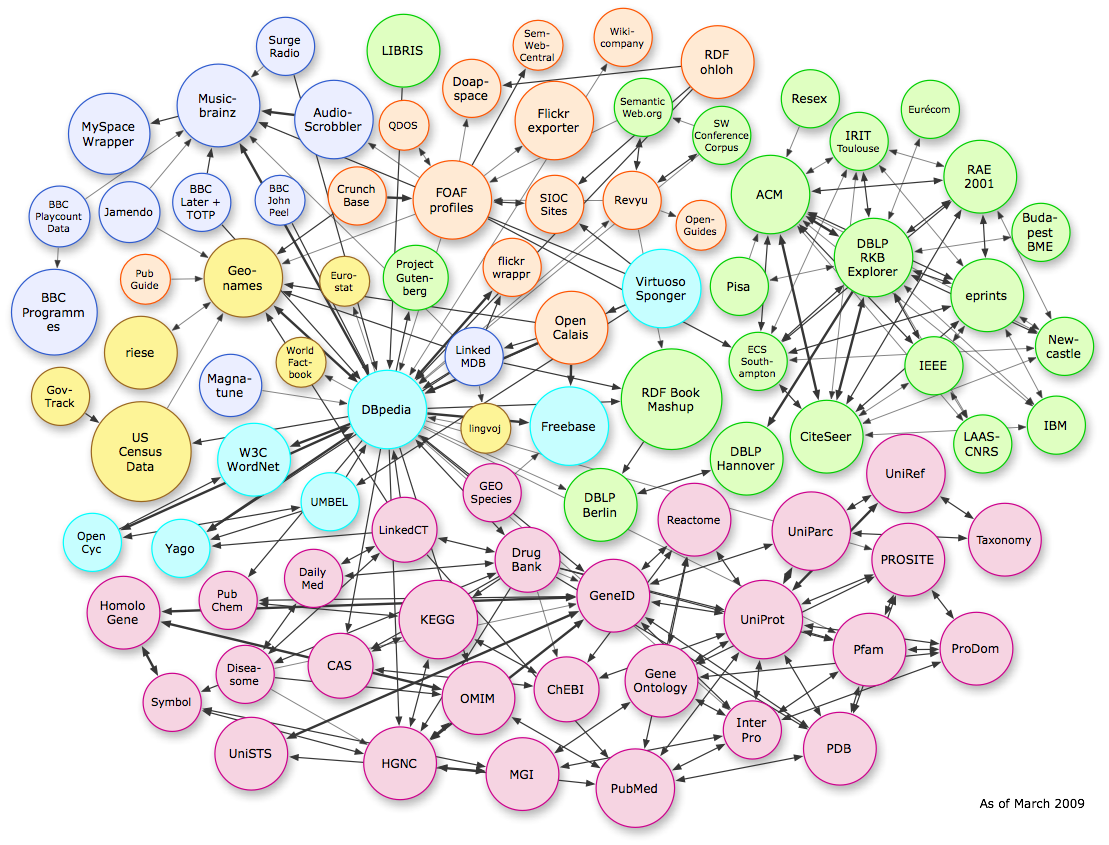
\includegraphics[width=\textwidth]{images/introduction/lod-cloud-2009-03-05}
        \end{subfigure}
        \begin{subfigure}{.325\textwidth}
            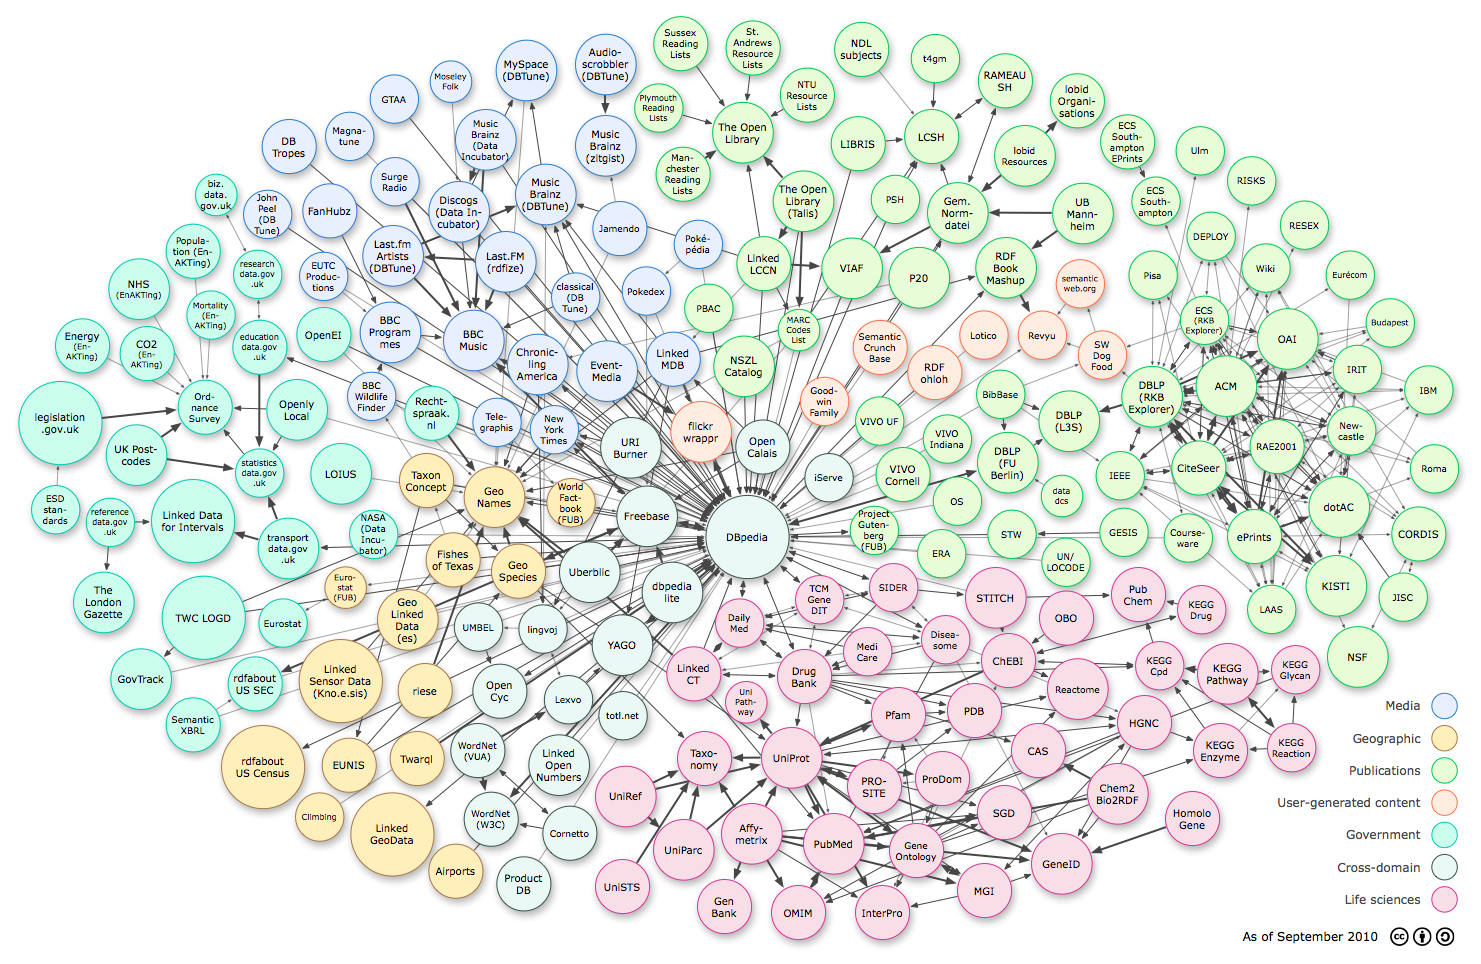
\includegraphics[width=\textwidth]{images/introduction/lod-cloud-2010-09-22}
        \end{subfigure}
        \begin{subfigure}{.365\textwidth}
            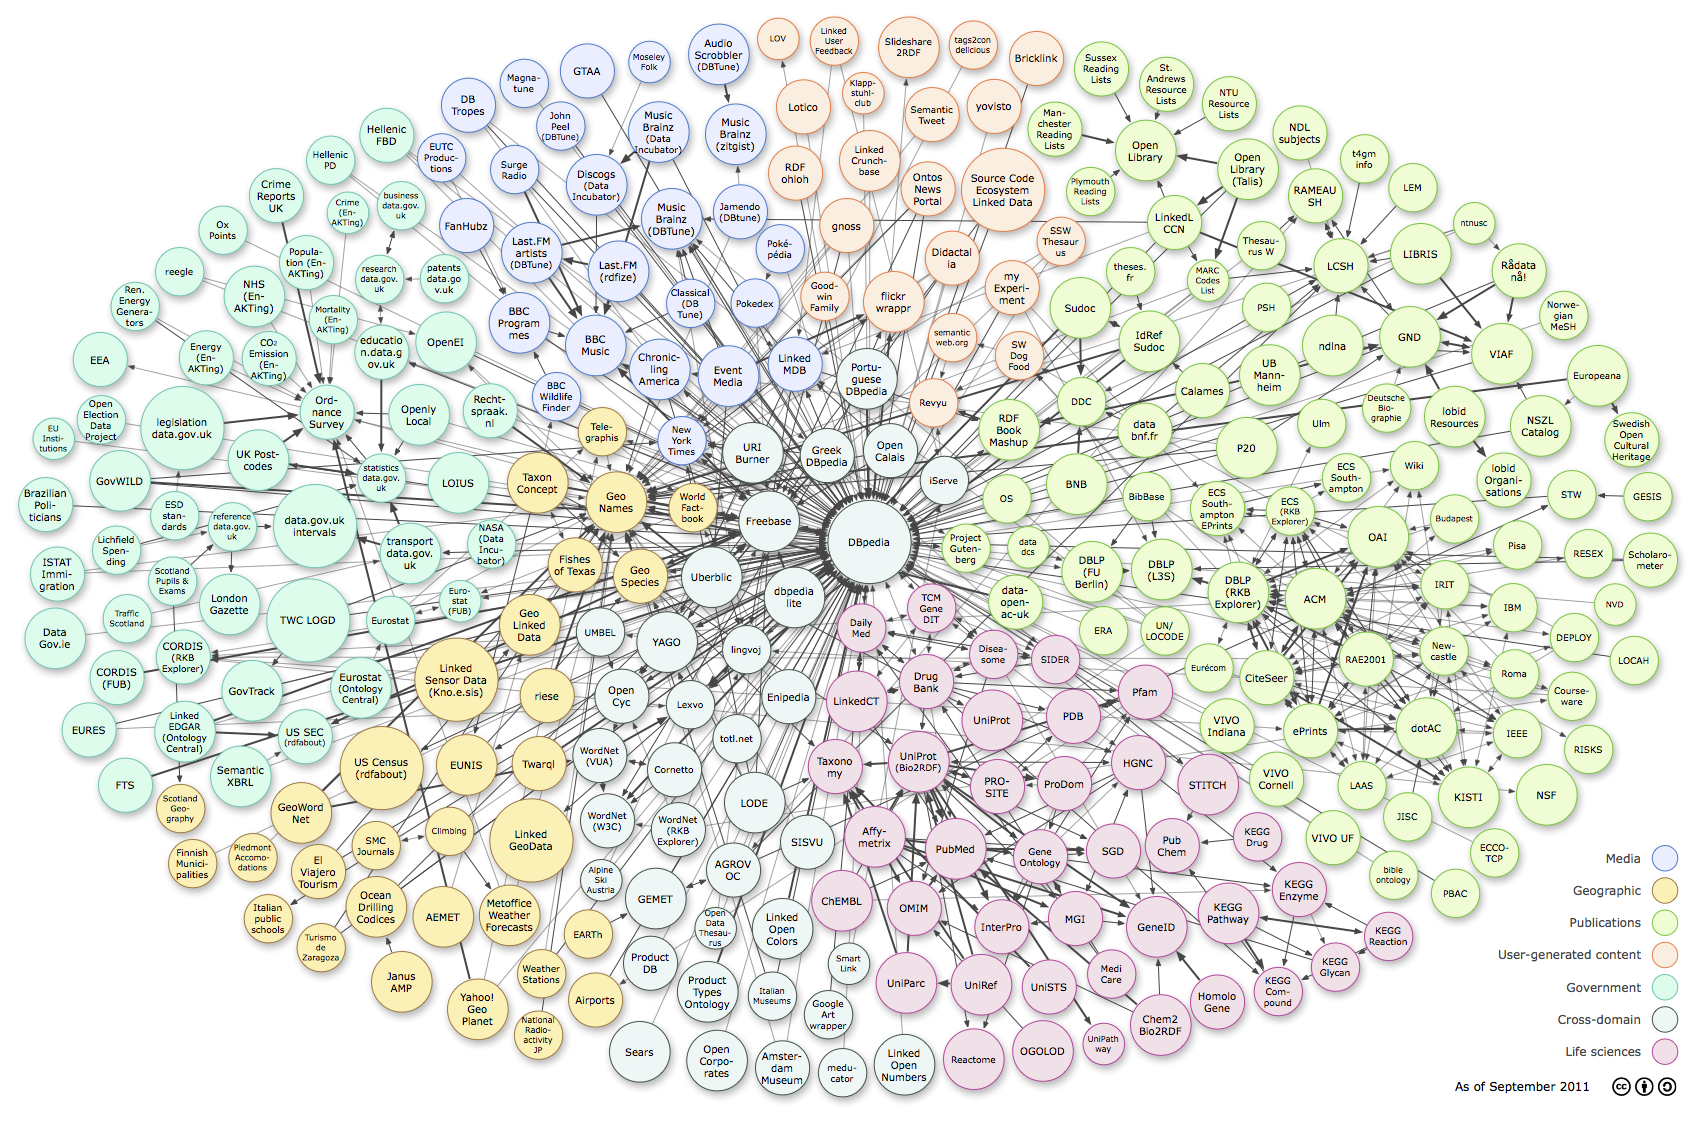
\includegraphics[width=\textwidth]{images/introduction/lod-cloud-2011-09-19}
        \end{subfigure}
        \begin{subfigure}{.45\textwidth}
            \includegraphics[width=\textwidth]{images/introduction/lod-cloud-2014-08-30}
        \end{subfigure}
    \end{figure}

    {\tiny Linking Open Data cloud diagram 2014, by Max Schmachtenberg, Christian Bizer, Anja Jentzsch and Richard Cyganiak. \url{http://lod-cloud.net/}}
}

\frame{
    \frametitle{How to Discover and Consume Web Data ?}
    \begin{columns}[c]
        \column{.5\textwidth}
        \begin{block}{Obstacles}
            \begin{itemize}
                \item Structure and vocabulary of the data change over time
                \item Schema is generally unknown
            \end{itemize}
        \end{block}

        \column{.5\textwidth}
        \begin{block}{Accessing Information}
            \begin{itemize}
                \item Usefulness of Web Data is measured by the ease-of-access to the data
                \item Relevant results to one's information need
            \end{itemize}
        \end{block}
    \end{columns}
}

\frame{
    \frametitle{Creation of a Schema-like Data Structure}
    \begin{block}{Top-Down Schema: Ontologies}
        \begin{itemize}
            \item Data has a known structure\ldots
            \item \ldots but it does not keep up with the pace of Web Data evolution
        \end{itemize}
    \end{block}
    \uncover<2->{
        \begin{block}{Bottom-Up Schema: Graph Summarisation}
            \begin{itemize}
                \item Embraces the Semantic Web vision\ldots
                \item \ldots but is sensitive to data quality
            \end{itemize}
        \end{block}
    }
}

\subsection{Use Case}

\frame{
    \frametitle{Use Case: Assisted Query Editing}
    \begin{figure}
        \centering
        \resizebox{.9\textwidth}{!}{
            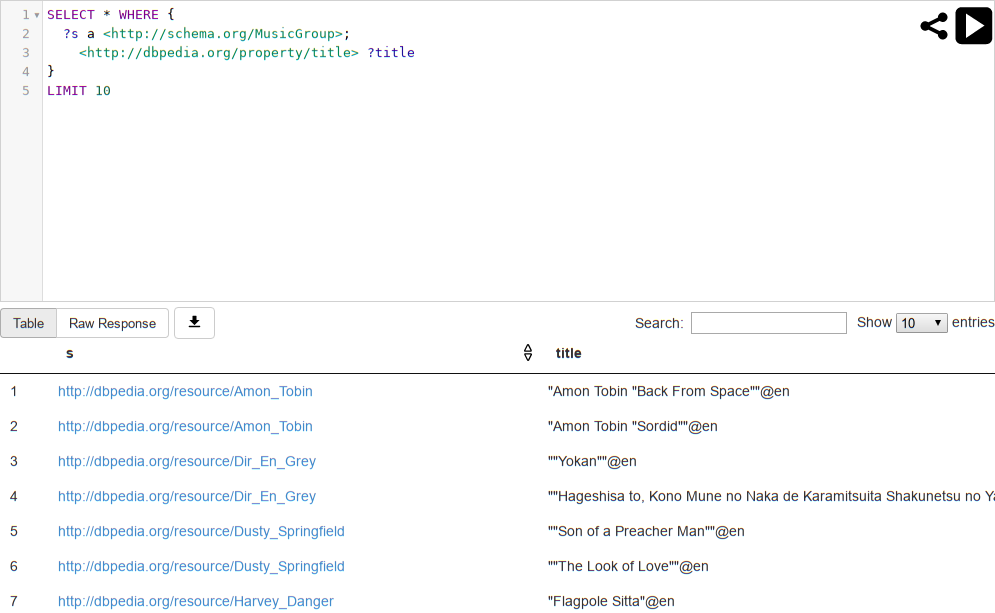
\includegraphics[scale=1]{images/introduction/use-case}
        }
    \end{figure}
}

\subsection{Challenges}

\frame{
    \frametitle{Challenges}
    \begin{block}{Graph Summarisation}
        \begin{itemize}
            \item How to generate a description of a dataset ?
            \item Scale to billions of triples
            \item How to measure the precision of the generated output ?
        \end{itemize}
    \end{block}
}
%% vim: et:sw=4


\AtBeginSection[]
{
    \frame{
        \frametitle{Table of Contents}
        \begin{multicols}{2}
            \tableofcontents[currentsection]
        \end{multicols}
    }
}

\section{Model}

\subsection{Graph Data Model}

\frame{
    \frametitle{Graph Data Model}
    \begin{figure}
        \centering
        \resizebox{.8\textwidth}{!}{
            \setbeamercovered{invisible}
\begin{tikzpicture}[->,>=stealth',node distance=2cm]
    \node[draw,circle] (d1) {$D_1$};
    \node[draw,circle,right of = d1,xshift=2cm] (d2) {$D_2$};
    
    \node[below of = d1,yshift=.5cm,xshift=-1.5cm] (ls) {};
    \node[below of = d2,yshift=.5cm,xshift=2.2cm] (le) {};
    
    \node[draw,circle,below of = d1,yshift=-1cm] (e11) {};
    \node[draw,circle,below right of = e11,yshift=.5cm] (e12) {};
    \node[draw,circle,below left of = e11,xshift=1cm] (e13) {};
    
    \node[draw,circle,below of = d2,yshift=-1cm] (e21) {};
    \node[draw,circle,below right of = e21] (e22) {};
    \node[draw,circle,below left of = e21,xshift=1cm,yshift=.2cm] (e23) {};
    
    \node[text width=3.56cm,inner sep=0pt,below of = d1,yshift=-1.75cm,xshift=.25cm] (d1it) {};
    \draw[dashed,thick] (d1it) ellipse (1.75cm and 1.1cm);
    
    \node[text width=3.56cm,inner sep=0pt,below of = d2,yshift=-1.75cm,xshift=.5cm] (d2it) {};
    \draw[dashed,thick] (d2it) ellipse (1.75cm and 1.1cm);
    
    \path[every node/.style={fill=white,font=\footnotesize}]
    (d1)	edge[bend left] node {$p_1$} (d2)
    (d2)	edge node {$p_2$} (d1)
    		edge[bend left] node {$p_3$} (d1)
    
    (ls) edge[-,very thick,dashed] (le)
    
    (e11)	edge (e13)
    (e12)	edge (e11)
    
    (e21)	edge (e22)
    			edge[bend right] node {$p_1$}  (e11)
    (e23) edge (e22)
    (e22)	edge[bend left] node[near end] {$p_2$} (e12)
    			edge[bend left] node {$p_3$} (e13)
    
    (d1.west) edge[-,dotted] (d1it.west)
    (d1.east) edge[-,dotted] (d1it.east)
    
    (d2.west) edge[-,dotted] (d2it.west)
    (d2.east) edge[-,dotted] (d2it.east)
    ;
\end{tikzpicture}
\setbeamercovered{transparent}
%% vim: et:sw=4

        }
        \caption{The graph data abstract model}
    \end{figure}
}

\subsection{Entity Model}

\frame{
    \frametitle{Entity Model}
    \begin{columns}[c]
        \column{.6\textwidth}
        \begin{figure}
            \centering
            \resizebox{\textwidth}{!}{
                \begin{tikzpicture}[->,>=stealth',node distance=3.5cm]
    \node [red,draw,circle] (n2) {$v_1$};
    \node [draw,circle,below of = n2,yshift=-1cm] (n1) {$v_2$};
    \node [blue,draw,circle,right of = n2] (n3) {$v_3$};
    \node [draw,circle,right of = n3] (n6) {$v_6$};
    \node [draw,circle,below of = n6,yshift=-1cm] (n4) {$v_4$};
    \node [draw,circle,below of = n2,yshift=1.25cm] (person) {Person};
    \node [draw,circle,below of = n1] (ren) {Renaud};
    \node [draw,circle,above of = n2] (ste) {St\'ephane};
    \node [draw,circle,right of = n4] (n5) {$v_5$};
    \node [draw,circle,right of = n6] (n7) {$v_7$};
    \node [draw,circle,above right of = n4,xshift=-.7cm] (place) {Place};
    \node [draw,circle,above of = n7,yshift=0cm] (country) {Country};
    \node [draw,circle,below of = n4] (deri) {DERI};
    \node [draw,circle,below of = n5] (fbk) {FBK};
    \node [draw,circle,above left of = n3,xshift=1cm] (city) {City};
    \node [draw,circle,above right of = n3,xshift=-1cm] (gal) {Galway};
    \node [draw,circle,right of = n7] (rome) {Rome};
    \node [draw,circle,above of = n6] (ire) {Ireland};

    \path
        (n7) edge node[fill=white] {capital} (rome)
        (n6) edge node[fill=white] {label} (ire)

        (n3) edge node[fill=white] {label} (gal)
        (n3) edge node[fill=white] {type} (city)

        (n4) edge node[fill=white] {label} (deri)
        (n5) edge node[fill=white] {label} (fbk)

        (n6) edge node[fill=white] {type} (country)
        (n7) edge node[fill=white] {type} (country)

        (n4) edge node[fill=white] {type} (place)
        (n5) edge node[fill=white] {type} (place)
        (n6) edge node[fill=white] {type} (place)
        (n7) edge node[fill=white] {type} (place)

        (n3) edge node[fill=white] {location} (n6)
        (n4) edge node[fill=white] {location} (n6)
        (n5) edge node[fill=white] {location} (n7)
        (n1) edge node[fill=white] {name} (ren)
        (n2) edge node[fill=white] {name} (ste)
        (n1) edge node[fill=white] {type} (person)
        (n2) edge node[fill=white] {type} (person)
        (n1) edge node[fill=white] {lives} (n3)
        (n1) edge node[fill=white] {works} (n4)
        (n2) edge node[fill=white] {lives} (n3)
        (n2) edge[near end] node[fill=white] {works} (n4)
    ;
\end{tikzpicture}
%% vim: et:sw=4

            }
            \caption{An entity graph describing people, places, and their relationships.}
        \end{figure}

        \column{.4\textwidth}
        \begin{figure}
            \centering
            \resizebox{!}{.18\textheight}{
                \begin{subfigure}{\textwidth}
                    \begin{tikzpicture}[->, >=stealth', node distance=2.5cm]
    \node [red,draw, circle,font=\footnotesize] (n0) {$v_1$};
    \node [draw, circle, above left of = n0,font=\footnotesize] (n1) {Person};
    \node [draw, circle, above right of = n0,font=\footnotesize] (n2) {Stephane};
    \node [draw, circle, below left of = n0,font=\footnotesize] (n3) {$v_3$};
    \node [draw, circle, below right of = n0,font=\footnotesize] (n4) {$v_4$};

    \path[every node/.style={fill=white,font=\scriptsize}]
        (n0) edge node {name} (n2)
        (n0) edge node {works} (n4)
        (n0) edge node {lives} (n3)
        (n0) edge node {type} (n1);
\end{tikzpicture}
%% vim: et:sw=4

                \end{subfigure}
            }
            \quad
            \resizebox{!}{.18\textheight}{
                \begin{subfigure}{\textwidth}
                    \begin{tikzpicture}[->, >=stealth', node distance=2.5cm]
    \node [blue,draw, circle,font=\footnotesize] (n0) {$v_3$};
    \node [draw, circle, above left of = n0,font=\footnotesize] (n1) {City};
    \node [draw, circle, above right of = n0,font=\footnotesize] (n2) {Galway};
    \node [draw, circle, below of = n0,font=\footnotesize] (n3) {$v_6$};

    \path[every node/.style={fill=white,font=\scriptsize}]
        (n0) edge node {label} (n2)
        (n0) edge node {location} (n3)
        (n0) edge node {type} (n1);
\end{tikzpicture}
%% vim: et:sw=4

                \end{subfigure}
            }
            \caption{Entity Descriptions}
        \end{figure}
    \end{columns}
}
%% vim: et:sw=4


\section{Graph Summarisation}

\subsection{Overview}

\frame{
    \frametitle{Overview}
    \begin{figure}
        \centering
        \begin{subfigure}[b]{.5\textwidth}
            \centering
            \resizebox{\textwidth}{!}{
                \begin{tikzpicture}[->, >=stealth', node distance=2.5cm]
\node[draw, circle] (n0) {$v_0$};
\node[draw, circle, below of = n0] (n01) {Person};
\node[draw, circle, above of = n0] (n02) {Alice};

\node[draw, circle, right of = n0] (n1) {$v_1$};
\node[draw, circle, below of = n1] (n11) {Person};
\node[draw, circle, above of = n1] (n12) {Bob};

\node[draw, circle, right of = n1] (nn) {$v_n$};
\node[draw, circle, below of = nn] (nn1) {Person};
\node[draw, circle, above of = nn] (nn2) {Zed};

\path[every node/.style={fill=white,font=\footnotesize}]
  (n0) edge node {name} (n02)
  (n0) edge node {type} (n01)

  (n1) edge node {name} (n12)
  (n1) edge node {type} (n11)

  (nn) edge node {name} (nn2)
  (nn) edge node {type} (nn1)
  (nn) edge[dotted, thick,-] (n1)
;
\end{tikzpicture}
%% vim: et:sw=4

            }
            \caption{An entity graph about people}
        \end{subfigure}
        \qquad
        \begin{subfigure}[b]{.4\textwidth}
            \centering
            \resizebox{.35\textwidth}{!}{
                \begin{tikzpicture}[->, >=stealth', node distance=2.5cm]
\node[draw, circle] (n0) {$u_0$};
\node[draw, circle, below of = n0] (n01) {Person};
\node[draw, circle, above of = n0] (n02) {$*$};

\path[every node/.style={fill=white,font=\footnotesize}]
  (n0) edge node {name} (n02)
  (n0) edge node {type} (n01)
;
\end{tikzpicture}
%% vim: et:sw=4

            }
            \caption{A possible summary}
        \end{subfigure}
        \caption{Summarising an entity graph}
    \end{figure}
}

\subsection{Model}

\frame[plain]{
    \frametitle{Graph Summary}
    \begin{definition}
        A graph is the \textbf{summary} of another graph if there is a \textbf{homomorphism} from the \emph{latter} to the \emph{former} with respect to a \textbf{relation}.
    \end{definition}
    \hfill\begin{minipage}{\dimexpr\textwidth-1cm}
        \begin{block}{Summarisation Relation}
            \begin{itemize}
                \item Mapping between the nodes of two graphs, based on \emph{features} of the graph
            \end{itemize}
        \end{block}
        \begin{block}{Graph Homomorphism}
            \begin{itemize}
                \item With respect to the summarisation relation, each edge of the graph is mapped to an edge(s) of the summary
            \end{itemize}
        \end{block}
    \end{minipage}
}

\frame{
    \frametitle{Graph Homomorphism}
    \begin{columns}[c]
        \column{.45\textwidth}
        \begin{definition}
            A graph is homomorphic to another if all of its edges do exist in that other graph for a given relation.
        \end{definition}

        \column{.6\textwidth}
        \begin{example}
            \begin{figure}
                \centering
                \resizebox{\textwidth}{!}{
                    \setbeamercovered{invisible}
\begin{tikzpicture}[->,>=stealth',node distance=2.25cm]
    \node [draw,circle] (1) {1};
    \node [draw,circle,below left of = 1] (2) {2};
    \node [draw,circle,below right of = 1] (3) {3};
    \node [draw,circle,above of = 1] (4) {4};

    \node [draw,circle,right of = 1,xshift=2cm,yshift=-1cm] (a) {a};
    \node [draw,circle,above of = a] (b) {b};

    % first edge
    \uncover<2-3>{
        \path[red highlight edge]
            (2) edge (1)
            ;
        \node [draw,circle, red highlight node] (1) {1};
        \node [draw,circle,below left of = 1, red highlight node] (2) {2};
    }
    \uncover<3-3>{
        \path[green highlight edge]
            (1) edge (b)
            (2) edge [bend left=10] (a)
            ;
        \path[red highlight edge]
            (b) edge (a)
            ;
        \node [red highlight node, draw,circle,right of = 1,xshift=2cm,yshift=-1cm] (a) {a};
        \node [red highlight node, draw,circle,above of = a] (b) {b};
    }

    % second edge
    \uncover<4-5>{
        \path[red highlight edge]
            (3) edge (1)
            ;
        \node [draw,circle, red highlight node] (1) {1};
        \node [draw,circle,below right of = 1, red highlight node] (3) {3};
    }
    \uncover<5-5>{
        \path[green highlight edge]
            (1) edge (b)
            (3) edge (a)
            ;
        \path[red highlight edge]
            (b) edge (a)
            ;
        \node [red highlight node, draw,circle,right of = 1,xshift=2cm,yshift=-1cm] (a) {a};
        \node [red highlight node, draw,circle,above of = a] (b) {b};
    }

    % third edge
    \uncover<6-7>{
        \path[red highlight edge]
            (1) edge (4)
            ;
        \node [draw,circle, red highlight node] (1) {1};
        \node [draw,circle,above of = 1, red highlight node] (4) {4};
    }
    \uncover<7-7>{
        \path[green highlight edge]
            (1) edge (b)
            (4) edge (b)
            ;
        \path[red highlight edge]
            (b) edge[loop] (b)
            ;
        \node [red highlight node, draw,circle,above of = a] (b) {b};
    }

    \path[every node/.style={fill=white,font=\footnotesize}]
        (1) edge[->] (4)
        (2) edge (1)
        (3) edge (1)
        (a) edge (b)
        (b) edge[loop] (b)
        (1) edge [dotted] node {$R$} (b)
        (4) edge [dotted] node {$R$} (b)
        (2) edge [dotted,bend left=10] node[near start] {$R$} (a)
        (3) edge [dotted] node {$R$} (a);

\end{tikzpicture}
\setbeamercovered{transparent}
%% vim: et:sw=4

                }
            \end{figure}
        \end{example}
    \end{columns}
}

\subsection{Precise Graph Summary}

\frame{
    \frametitle{Precise Graph Summary}
    \begin{columns}[c]
        \column{.55\textwidth}
        \begin{block}{Inevitability of Precision Loss}
            \begin{itemize}
                \item A summary is precise if every path in the graph do exist
                \item Creating such a summary is impractical due to the data's heterogeneity
            \end{itemize}
        \end{block}

        \column{.5\textwidth}
        \begin{figure}
            \centering
            \resizebox{\textwidth}{!}{
                \begin{tikzpicture}
    \begin{loglogaxis}[
                grid=major,
                        xlabel=number of documents (\emph{log}),
                        ylabel=probability (\emph{log}),
                ]
        \addplot[red, domain=1:100,ultra thick] {0.00257344864/(x^1.913581)};
        \addlegendentry{$\alpha =  1.91$}
        \addplot+[only marks, mark size=1pt,mark=star, blue] table[x index=1,y index=0] {images/summarisation/basic-namespace-stats-probability};
	\end{loglogaxis}
\end{tikzpicture}

            }
            \caption{Ontology probability distribution}
        \end{figure}
    \end{columns}
}

\subsection{Approximate Graph Summaries}

\frame{
    \frametitle{Approximate Graph Summaries}
    \begin{block}{Why approximate a summary ?}
        \begin{itemize}
            \item Web Data is too heterogeneous for its structure to be captured perfectly
            \item Summarisation needs to scale to large graphs
        \end{itemize}
    \end{block}
    \begin{block}{Features}
        \begin{itemize}
            \item Types
            \item Attributes (incoming and/or outgoing)
        \end{itemize} 
    \end{block}

    %\uncover<2->{
        %\begin{block}{Studied Summaries}
            %\begin{columns}[c]
                %\column{.5\textwidth}
                %\begin{itemize}
                    %\item Unique Type Summary
                    %\item Types Summary
                    %\item Attributes Summary
                %\end{itemize} 

                %\column{.6\textwidth}
                %\begin{itemize}
                    %\item Types \& Attributes Summary
                    %\item IO Attributes Summary
                    %\item IO Attributes Types Summary
                %\end{itemize} 
            %\end{columns}
        %\end{block}
    %}
}

\frame[shrink]{
    \frametitle{Example: Types Summary}
    \vspace{2em}
    \begin{description}
        \item[Relation:] set of types associated to a node
    \end{description}
    \vspace{-1em}
    \begin{columns}[c]
        \column{.6\textwidth}
        \begin{figure}[b]
            \centering
            \resizebox{.9\textwidth}{!}{
                \setbeamercovered{invisible}
\begin{tikzpicture}[->,>=stealth',node distance=3.5cm]
    \node [draw,circle] (n2) {$v_1$};
    \node [draw,circle,below of = n2,yshift=-1cm] (n1) {$v_2$};
    \node [draw,circle,right of = n2] (n3) {$v_3$};
    \node [draw,circle,right of = n3] (n6) {$v_6$};
    \node [draw,circle,below of = n6,yshift=-1cm] (n4) {$v_4$};
    \node [draw,circle,below of = n2,yshift=1.25cm] (person) {Person};
    \node [draw,circle,below of = n1] (ren) {Renaud};
    \node [draw,circle,above of = n2] (ste) {St\'ephane};
    \node [draw,circle,right of = n4] (n5) {$v_5$};
    \node [draw,circle,right of = n6] (n7) {$v_7$};
    \node [draw,circle,above right of = n4,xshift=-.7cm] (place) {Place};
    \node [draw,circle,above of = n7,yshift=0cm] (country) {Country};
    \node [draw,circle,below of = n4] (deri) {DERI};
    \node [draw,circle,below of = n5] (fbk) {FBK};
    \node [draw,circle,above left of = n3,xshift=1cm] (city) {City};
    \node [draw,circle,above right of = n3,xshift=-1cm] (gal) {Galway};
    \node [draw,circle,above right of = n7] (rome) {Rome};
    \node [draw,circle,above of = n6] (ire) {Ireland};

    \uncover<2-2>{
        \node [draw,circle,below of = n2,yshift=1.25cm, green highlight node] (person) {Person};
        \path[green highlight edge]
            (person) edge (n2) edge (n1)
            ;
        \node [draw,circle, red highlight node] (n2) {$v_1$};
        \node [draw,circle,below of = n2,yshift=-1cm, red highlight node] (n1) {$v_2$};
    }

    \uncover<3-3>{
        \node [draw,circle,above left of = n3,xshift=1cm, green highlight node] (city) {City};
        \path[green highlight edge]
            (n3) edge (city)
            ;
        \node [draw,circle,right of = n2, red highlight node] (n3) {$v_3$};
    }

    \uncover<4-4>{
        \node [draw,circle,above right of = n4,xshift=-.7cm, green highlight node] (place) {Place};
        \path[green highlight edge]
            (n4) edge (place)
            (n5) edge (place)
            ;
        \node [draw,circle,below of = n6,yshift=-1cm, red highlight node] (n4) {$v_4$};
        \node [draw,circle,right of = n4, red highlight node] (n5) {$v_5$};
    }

    \uncover<5-5>{
        \node [draw,circle,above of = n7,yshift=0cm, green highlight node] (country) {Country};
        \node [draw,circle,above right of = n4,xshift=-.7cm, green highlight node] (place) {Place};
        \path[green highlight edge]
            (place) edge (n6) edge (n7)
            (country) edge (n6) edge (n7)
            ;
        \node [draw,circle,right of = n3, red highlight node] (n6) {$v_6$};
        \node [draw,circle,right of = n6, red highlight node] (n7) {$v_7$};
    }

    \uncover<6-6>{
        \node [draw,circle,below of = n1, red highlight node] (ren) {Renaud};
        \node [draw,circle,above of = n2, red highlight node] (ste) {St\'ephane};
        \node [draw,circle,below of = n4, red highlight node] (deri) {DERI};
        \node [draw,circle,below of = n5, red highlight node] (fbk) {FBK};
        \node [draw,circle,above right of = n3,xshift=-1cm, red highlight node] (gal) {Galway};
        \node [draw,circle,above right of = n7, red highlight node] (rome) {Rome};
        \node [draw,circle,above of = n6, red highlight node] (ire) {Ireland};
    }

    \uncover<7-7>{
        \node [draw,circle, red highlight node] (n2) {$v_1$};
        \node [draw,circle,above of = n2, red highlight node] (ste) {St\'ephane};
        \draw [red highlight edge] (n2) edge node[fill=white] {name} (ste);
    }

    \uncover<8-8>{
        \node [draw,circle, red highlight node] (n2) {$v_1$};
        \node [draw,circle,right of = n2, red highlight node] (n3) {$v_3$};
        \draw [red highlight edge] (n2) edge node[fill=white] {lives} (n3);
    }

    \path
        (n7) edge node[fill=white] {capital} (rome)
        (n6) edge node[fill=white] {label} (ire)

        (n3) edge node[fill=white] {label} (gal)
        (n3) edge node[fill=white] {type} (city)

        (n4) edge node[fill=white] {label} (deri)
        (n5) edge node[fill=white] {label} (fbk)

        (n6) edge node[fill=white] {type} (country)
        (n7) edge node[fill=white] {type} (country)

        (n4) edge node[fill=white] {type} (place)
        (n5) edge node[fill=white] {type} (place)
        (n6) edge node[fill=white] {type} (place)
        (n7) edge node[fill=white] {type} (place)

        (n3) edge node[fill=white] {location} (n6)
        (n4) edge node[fill=white] {location} (n6)
        (n5) edge node[fill=white] {location} (n7)
        (n1) edge node[fill=white] {name} (ren)
        (n2) edge node[fill=white] {name} (ste)
        (n1) edge node[fill=white] {type} (person)
        (n2) edge node[fill=white] {type} (person)
        (n1) edge node[fill=white] {lives} (n3)
        (n1) edge node[fill=white] {works} (n4)
        (n2) edge node[fill=white] {lives} (n3)
        (n2) edge[near end] node[fill=white] {works} (n4)
    ;
\end{tikzpicture}
\setbeamercovered{transparent}
%% vim: et:sw=4

            }
            \caption{An entity graph describing people, places, and their relationships.}
        \end{figure}

        \column{.4\textwidth}
        \begin{figure}[b]
            \centering
            \resizebox{.9\textwidth}{!}{
                \setbeamercovered{invisible}
\begin{tikzpicture}[->,>=stealth',node distance=4cm]
    \uncover<2-2,7-8>{
        \node [draw,circle, red highlight node] (h1) {$S_1$};
    }
    \uncover<2->{
        \node [draw,circle] (h1) {$S_1$};
    }

    \uncover<3-3,8-8>{
        \node [draw,circle,above right of = h1, red highlight node] (h2) {$S_2$};
    }
    \uncover<3->{
        \node [draw,circle,above right of = h1] (h2) {$S_2$};
    }

    \uncover<4-4>{
        \node [draw,circle,below right of = h1, red highlight node] (h3) {$S_3$};
    }
    \uncover<4->{
        \node [draw,circle,below right of = h1] (h3) {$S_3$};
    }

    \uncover<5-5>{
        \node [draw,circle,above right of = h3, red highlight node] (h4) {$S_4$};
    }
    \uncover<5->{
        \node [draw,circle,above right of = h3] (h4) {$S_4$};
    }

    \uncover<2-2>{
        \node [draw,circle,above of = h1, green highlight node] (person) {Person};
    }
    \uncover<2->{
        \node [draw,circle,above of = h1] (person) {Person};
    }

    \uncover<3-3>{
        \node [draw,circle,above of = h2, green highlight node] (city) {City};
    }
    \uncover<3->{
        \node [draw,circle,above of = h2] (city) {City};
    }

    \uncover<5-5>{
        \node [draw,circle,above of = h4, green highlight node] (country) {Country};
    }
    \uncover<5->{
        \node [draw,circle,above of = h4] (country) {Country};
    }

    \uncover<4-5>{
        \node [draw,circle,below right of = h4,xshift=-1cm, green highlight node] (place) {Place};
    }
    \uncover<4->{
        \node [draw,circle,below right of = h4,xshift=-1cm] (place) {Place};
    }

    \uncover<6-7>{
        \node [draw,circle,below of = h2,yshift=1cm, red highlight node] (c2) {$\varnothing$};
    }
    \uncover<6->{
        \node [draw,circle,below of = h2,yshift=1cm] (c2) {$\varnothing$};
    }

    %%%
    %%% Edges
    %%%
    \uncover<2-2>{
        \draw [green highlight edge] (h1) edge node[fill=white] {type} (person);
    }
    \uncover<2->{
        \draw (h1) edge node[fill=white] {type} (person);
    }

    \uncover<3-3>{
        \draw [green highlight edge] (h2) edge node[fill=white] {type} (city);

    }
    \uncover<3->{
        \draw (h1) (h2) edge node[fill=white] {type} (city);
    }

    \uncover<4-4>{
        \draw [green highlight edge] (h3) edge node[fill=white] {type} (place);
    }
    \uncover<4->{
        \draw (h3) edge node[fill=white] {type} (place);
    }

    \uncover<5-5>{
        \draw [green highlight edge] (h4) edge node[fill=white] {type} (place);
    }
    \uncover<5->{
        \draw (h4) edge node[fill=white] {type} (place);
    }

    \uncover<5-5>{
        \draw [green highlight edge] (h4) edge node[near end,fill=white] {type} (country);
    }
    \uncover<5->{
        \draw (h4) edge node[near end,fill=white] {type} (country);
    }

    \uncover<7-7>{
        \draw [red highlight edge] (h1) edge node[fill=white] {name} (c2);
    }
    \uncover<7->{
        \draw (h1) edge node[fill=white] {name} (c2);
    }

    \uncover<8-8>{
        \draw [red highlight edge] (h1) edge[bend left] node[fill=white] {lives} (h2);
    }
    \uncover<8->{
        \draw (h1) edge[bend left] node[fill=white] {lives} (h2);
    }

    \uncover<9->{
        \path
            (h3) edge node[fill=white] {label} (c2)
            (h2) edge node[fill=white] {label} (c2)
            (h4) edge[bend right] node[fill=white] {label} (c2)
            (h4) edge[bend left] node[fill=white] {capital} (c2)

            (h3) edge node[fill=white] {type} (place)
            (h1) edge[bend right] node[fill=white] {works} (h3)
            (h2) edge[bend left] node[fill=white] {location} (h4)
            (h3) edge[bend right] node[fill=white] {location} (h4)
            ;
    }
\end{tikzpicture}
\setbeamercovered{transparent}
%% vim: et:sw=4

            }
            \caption{Types summary of the entity graph.}
        \end{figure}
    \end{columns}
}

\subsection{Implementations}

\frame[shrink]{
    \frametitle{Implementations}
    \vspace{.5cm}
    \begin{block}{Algorithm}
        \begin{enumerate}
            \item Entity description (group operator)
            \item Nodes mapping (object invention)
            \item Edges materialization (join operator)
        \end{enumerate}
    \end{block}
    \uncover<2->{
        \begin{columns}[c]
            \column{.5\textwidth}
            \begin{block}{SPARQL}
                \begin{alert}{Performance:}
                    Timeout for graphs above 20M triples.
                \end{alert} 
                \\
                \begin{alert}{Pros:}
                    Leverage endpoint for optimizing queries.
                \end{alert}
                \\
                \begin{alert}{Const:}
                    Bounded by the expressivity of SPARQL.
                \end{alert}
            \end{block}

            \column{.5\textwidth}
            \begin{block}{MapReduce}
                \begin{alert}{Performance:}
                    Scale to large graphs up to 50B triples.
                \end{alert} 
                \\
                \begin{alert}{Pros:}
                    More possiblities for optimisations.
                \end{alert}
                \\
                \begin{alert}{Cons:}
                    Cluster maintenance.
                \end{alert}
            \end{block}
        \end{columns}
    }
}
%% vim: et:sw=4


\section{Precision Model}

\subsection{Overview}

\frame{
    \frametitle{Loss of Precision with the Types Summary}
    \begin{columns}[c]
        \column{.6\textwidth}
        \begin{figure}
            \centering
            \resizebox{.9\textwidth}{!}{
                \setbeamercovered{invisible}
\begin{tikzpicture}[->,>=stealth',node distance=3.5cm]
    \node [draw,circle] (n2) {$v_1$};
    \node [draw,circle,below of = n2,yshift=-1cm] (n1) {$v_2$};
    \node [draw,circle,right of = n2] (n3) {$v_3$};
    \node [draw,circle,right of = n3] (n6) {$v_6$};
    \node [draw,circle,below of = n6,yshift=-1cm] (n4) {$v_4$};
    \node [draw,circle,below of = n2,yshift=1.25cm] (person) {Person};
    \node [draw,circle,below of = n1] (ren) {Renaud};
    \node [draw,circle,above of = n2] (ste) {St\'ephane};
    \node [draw,circle,right of = n4] (n5) {$v_5$};
    \node [draw,circle,right of = n6] (n7) {$v_7$};
    \node [draw,circle,above right of = n4,xshift=-.7cm] (place) {Place};
    \node [draw,circle,above of = n7,yshift=0cm] (country) {Country};
    \node [draw,circle,below of = n4] (deri) {DERI};
    \node [draw,circle,below of = n5] (fbk) {FBK};
    \node [draw,circle,above left of = n3,xshift=1cm] (city) {City};
    \node [draw,circle,above right of = n3,xshift=-1cm] (gal) {Galway};
    \node [draw,circle,above right of = n7] (rome) {Rome};
    \node [draw,circle,above of = n6] (ire) {Ireland};

    \uncover<5-6>{
        \node [red highlight node,draw,circle,below of = n6,yshift=-1cm] (n4) {$v_4$};
        \node [red highlight node,draw,circle,right of = n3] (n6) {$v_6$};
        \draw[red highlight edge] (n4) edge (n6);

        \node [red highlight node,draw,circle,right of = n6] (n7) {$v_7$};
        \node [red highlight node,draw,circle,above right of = n7] (rome) {Rome};
        \draw [red highlight edge, dotted] (n7) edge node[fill=white] {capital} (rome);
    }

    \uncover<5-5>{
        \node [red highlight node,draw,circle] (n2) {$v_1$};
        \draw[red highlight edge] (n2) edge (n4);
    }

    \uncover<6-6>{
        \node [red highlight node,draw,circle,below of = n2,yshift=-1cm] (n1) {$v_2$};
        \draw[red highlight edge] (n1) edge (n4);
    }

    \path
        (n7) edge node[fill=white] {capital} (rome)
        (n6) edge node[fill=white] {label} (ire)

        (n3) edge node[fill=white] {label} (gal)
        (n3) edge node[fill=white] {type} (city)

        (n4) edge node[fill=white] {label} (deri)
        (n5) edge node[fill=white] {label} (fbk)

        (n6) edge node[fill=white] {type} (country)
        (n7) edge node[fill=white] {type} (country)

        (n4) edge node[fill=white] {type} (place)
        (n5) edge node[fill=white] {type} (place)
        (n6) edge node[fill=white] {type} (place)
        (n7) edge node[fill=white] {type} (place)

        (n3) edge node[fill=white] {location} (n6)
        (n4) edge node[fill=white] {location} (n6)
        (n5) edge node[fill=white] {location} (n7)
        (n1) edge node[fill=white] {name} (ren)
        (n2) edge node[fill=white] {name} (ste)
        (n1) edge node[fill=white] {type} (person)
        (n2) edge node[fill=white] {type} (person)
        (n1) edge node[fill=white] {lives} (n3)
        (n1) edge node[fill=white] {works} (n4)
        (n2) edge node[fill=white] {lives} (n3)
        (n2) edge[near end] node[fill=white] {works} (n4)
    ;
\end{tikzpicture}
\setbeamercovered{transparent}
%% vim: et:sw=4

            }
            \caption{An entity graph describing people, places, and their relationships.}
        \end{figure}

        \column{.4\textwidth}
        \begin{figure}
            \centering
            \resizebox{.9\textwidth}{!}{
                \setbeamercovered{invisible}
\begin{tikzpicture}[->,>=stealth',node distance=4cm]
    \node [draw,circle] (h1) {$S_1$};
    \node [draw,circle,above right of = h1] (h2) {$S_2$};
    \node [draw,circle,below right of = h1] (h3) {$S_3$};
    \node [draw,circle,above right of = h3] (h4) {$S_4$};
    \node [draw,circle,above of = h1] (person) {Person};
    \node [draw,circle,above of = h2] (city) {City};
    \node [draw,circle,above of = h4] (country) {Country};
    \node [draw,circle,below right of = h4,xshift=-1cm] (place) {Place};
    \node [draw,circle,below of = h2,yshift=1cm] (c2) {$S_5$};

    \uncover<2-6>{
        \node [green highlight node,draw,circle] (h1) {$S_1$};
        \node [green highlight node,draw,circle,below right of = h1] (h3) {$S_3$};
        \draw [green highlight edge] (h1) edge[bend right] (h3);
    }
    \uncover<3-6>{
        \node [green highlight node,draw,circle,below right of = h1] (h3) {$S_3$};
        \node [green highlight node,draw,circle,above right of = h3] (h4) {$S_4$};
        \draw [green highlight edge] (h3) edge[bend right] (h4);
    }
    \uncover<4-6>{
        \node [green highlight node,draw,circle,above right of = h3] (h4) {$S_4$};
        \node [green highlight node,draw,circle,below of = h2,yshift=1cm] (c2) {$S_5$};
        \draw [green highlight edge] (h4) edge[bend left] (c2);
    }

    \path
        (h1) edge node[fill=white] {name} (c2)
        (h3) edge node[fill=white] {label} (c2)
        (h2) edge node[fill=white] {label} (c2)
        (h4) edge[bend right] node[fill=white] {label} (c2)
        (h4) edge[bend left] node[fill=white] {capital} (c2)

        (h1) edge node[fill=white] {type} (person)
        (h2) edge node[fill=white] {type} (city)
        (h4) edge node[near end,fill=white] {type} (country)
        (h4) edge node[fill=white] {type} (place)
        (h3) edge node[fill=white] {type} (place)
        (h1) edge[bend left] node[fill=white] {lives} (h2)
        (h1) edge[bend right] node[fill=white] {works} (h3)
        (h2) edge[bend left] node[fill=white] {location} (h4)
        (h3) edge[bend right] node[fill=white] {location} (h4)
        ;
\end{tikzpicture}
\setbeamercovered{transparent}
%% vim: et:sw=4

            }
            \caption{Types summary of the entity graph.}
        \end{figure}
    \end{columns}
}

\subsection{Model}

\frame{
    \frametitle{Ordering of Graph Summaries}
    \vspace{2em}
    \begin{block}{Partial Relation}
        \begin{figure}
            \centering
            \resizebox{.6\textwidth}{!}{
                \setbeamercovered{invisible}
\begin{tikzpicture}[->,>=stealth',node distance=3cm]
    \node (g) {$G$};
    \node[right of = g] (g1) {$\mathcal{S}_1$};
    \node[right of = g1] (g2) {$\mathcal{S}_2$};

    \uncover<2->{
        \draw[red] (g1) edge node[red,above] {$R_3$} (g2);
    }

    \path
        (g) edge node[above] {$R_1$} (g1)
        (g) edge [bend right=20] node[below] {$R_2$} (g2)
        ;
\end{tikzpicture}
\setbeamercovered{transparent}
%% vim: et:sw=4

            }
        \end{figure}
    \end{block}
    \vspace{-2em}
    \uncover<3->{
        \begin{block}{Graph Lattice}
            \begin{figure}
                \centering
                \resizebox{.8\textwidth}{!}{
                    \begin{tikzpicture}[->,>=stealth',node distance=2cm]
\node (base) {\emph{Infimum}};
\node[right of = base] (ioat) {$R_{ioat}$};
\node[right of = ioat] (ta1) {$R_{iat}$};
\node[above of = ta1] (at) {$R_{at}$};
\node[below of = ta1] (ioa) {$R_{ioa}$};
\node[right of = at] (t) {$R_t$};
\node[right of = ta1] (a) {$R_a$};
\node[right of = ioa] (a1) {$R_{ia}$};
\node[right of = t] (st) {$R_{ut}$};
\node[right of = a] (phantom) {};
\node[right of = phantom] (apex) {\emph{Supremum}};

\path
(base) edge (ioat)
(ioat) edge (ta1)
(ioat) edge (at)
(ioat) edge (ioa)
(at) edge (t)
(at) edge (a)
(ioa) edge (a)
(ioa) edge (a1)
(ta1) edge (t)
(ta1) edge (a1)
(t) edge (st)
(st) edge (apex)
(a) edge (apex)
(a1) edge (apex)
;
\end{tikzpicture}
%% vim: et:sw=4

                }
            \end{figure}
        \end{block}
    }
}

\frame{
    \frametitle{Model}
    \begin{block}{Comparison}
        \begin{itemize}
            \item Leverage the partial relation for ordering the summaries
            \item Compare a summary against the original graph
            \item Compute how many errors the summarisation committed
        \end{itemize}
    \end{block}
    \begin{block}{Error Classification}
        \begin{itemize}
            \item Connectivity
            \item Attribute and type
        \end{itemize}
    \end{block}
}

\frame{
    \frametitle{An Example:\\Evaluation of the Summary Precision}
    \begin{columns}[c]
        \column{.6\textwidth}
        \begin{figure}
            \centering
            \resizebox{.9\textwidth}{!}{
                \setbeamercovered{invisible}
\begin{tikzpicture}[->,>=stealth',node distance=3.5cm]
    \uncover<1-1>{
        \node [draw,circle] (n2) {$v_1$};
        \node [draw,circle,below of = n2,yshift=-1cm] (n1) {$v_2$};
        \node [draw,circle,right of = n2] (n3) {$v_3$};
        \node [draw,circle,right of = n3] (n6) {$v_6$};
        \node [draw,circle,below of = n6,yshift=-1cm] (n4) {$v_4$};
        \node [draw,circle,below of = n2,yshift=1.25cm] (person) {Person};
        \node [draw,circle,below of = n1] (ren) {Renaud};
        \node [draw,circle,above of = n2] (ste) {St\'ephane};
        \node [draw,circle,right of = n4] (n5) {$v_5$};
        \node [draw,circle,right of = n6] (n7) {$v_7$};
        \node [draw,circle,above right of = n4,xshift=-.7cm] (place) {Place};
        \node [draw,circle,above of = n7,yshift=0cm] (country) {Country};
        \node [draw,circle,below of = n4] (deri) {DERI};
        \node [draw,circle,below of = n5] (fbk) {FBK};
        \node [draw,circle,above left of = n3,xshift=1cm] (city) {City};
        \node [draw,circle,above right of = n3,xshift=-1cm] (gal) {Galway};
        \node [draw,circle,above right of = n7] (rome) {Rome};
        \node [draw,circle,above of = n6] (ire) {Ireland};

        \path
            (n7) edge node[fill=white] {capital} (rome)
            (n6) edge node[fill=white] {label} (ire)
    
            (n3) edge node[fill=white] {label} (gal)
            (n3) edge node[fill=white] {type} (city)
    
            (n4) edge node[fill=white] {label} (deri)
            (n5) edge node[fill=white] {label} (fbk)
    
            (n6) edge node[fill=white] {type} (country)
            (n7) edge node[fill=white] {type} (country)
    
            (n4) edge node[fill=white] {type} (place)
            (n5) edge node[fill=white] {type} (place)
            (n6) edge node[fill=white] {type} (place)
            (n7) edge node[fill=white] {type} (place)
    
            (n3) edge node[fill=white] {location} (n6)
            (n4) edge node[fill=white] {location} (n6)
            (n5) edge node[fill=white] {location} (n7)
            (n1) edge node[fill=white] {name} (ren)
            (n2) edge node[fill=white] {name} (ste)
            (n1) edge node[fill=white] {type} (person)
            (n2) edge node[fill=white] {type} (person)
            (n1) edge node[fill=white] {lives} (n3)
            (n1) edge node[fill=white] {works} (n4)
            (n2) edge node[fill=white] {lives} (n3)
            (n2) edge[near end] node[fill=white] {works} (n4)
        ;
    }

    \uncover<2->{
        \node [draw,circle] (n2) {7};
        \node [draw,circle,below of = n2,yshift=-1cm] (n1) {13};
        \node [draw,circle,right of = n2] (n3) {8};
        \node [draw,circle,right of = n3] (n6) {9};
        \node [draw,circle,below of = n6,yshift=-1cm] (n4) {14};
        \node [draw,circle,below of = n2,yshift=1.25cm] (person) {11};
        \node [draw,circle,below of = n1] (ren) {16};
        \node [draw,circle,above of = n2] (ste) {1};
        \node [draw,circle,right of = n4] (n5) {15};
        \node [draw,circle,right of = n6] (n7) {10};
        \node [draw,circle,above right of = n4,xshift=-.7cm] (place) {12};
        \node [draw,circle,above of = n7,yshift=0cm] (country) {5};
        \node [draw,circle,below of = n4] (deri) {17};
        \node [draw,circle,below of = n5] (fbk) {18};
        \node [draw,circle,above left of = n3,xshift=1cm] (city) {2};
        \node [draw,circle,above right of = n3,xshift=-1cm] (gal) {3};
        \node [draw,circle,above right of = n7] (rome) {6};
        \node [draw,circle,above of = n6] (ire) {4};

        \path
            (n7) edge node[fill=white] {capital} (rome)
            (n6) edge node[fill=white] {label} (ire)
    
            (n3) edge node[fill=white] {label} (gal)
            (n3) edge node[fill=white] {type} (city)
    
            (n4) edge node[fill=white] {label} (deri)
            (n5) edge node[fill=white] {label} (fbk)
    
            (n6) edge node[fill=white] {type} (country)
            (n7) edge node[fill=white] {type} (country)
    
            (n4) edge node[fill=white] {type} (place)
            (n5) edge node[fill=white] {type} (place)
            (n6) edge node[fill=white] {type} (place)
            (n7) edge node[fill=white] {type} (place)
    
            (n3) edge node[fill=white] {location} (n6)
            (n4) edge node[fill=white] {location} (n6)
            (n5) edge node[fill=white] {location} (n7)
            (n1) edge node[fill=white] {name} (ren)
            (n2) edge node[fill=white] {name} (ste)
            (n1) edge node[fill=white] {type} (person)
            (n2) edge node[fill=white] {type} (person)
            (n1) edge node[fill=white] {lives} (n3)
            (n1) edge node[fill=white] {works} (n4)
            (n2) edge node[fill=white] {lives} (n3)
            (n2) edge[near end] node[fill=white] {works} (n4)
        ;
    }
\end{tikzpicture}
\setbeamercovered{transparent}
%% vim: et:sw=4

            }
        \end{figure}

        \column{.4\textwidth}
        \begin{figure}
            \centering
            \resizebox{.9\textwidth}{!}{
                \setbeamercovered{invisible}
\begin{tikzpicture}[->,>=stealth',node distance=4cm]
    \uncover<1-1>{
        \node [draw,circle] (h1) {$S_1$};
        \node [draw,circle,above right of = h1] (h2) {$S_2$};
        \node [draw,circle,below right of = h1] (h3) {$S_3$};
        \node [draw,circle,above right of = h3] (h4) {$S_4$};
        \node [draw,circle,above of = h1] (person) {Person};
        \node [draw,circle,above of = h2] (city) {City};
        \node [draw,circle,above of = h4] (country) {Country};
        \node [draw,circle,below right of = h4,xshift=-1cm] (place) {Place};
        \node [draw,circle,below of = h2,yshift=1cm] (c2) {$\varnothing$};

        \path
            (h1) edge node[fill=white] {name} (c2)
            (h3) edge node[fill=white] {label} (c2)
            (h2) edge node[fill=white] {label} (c2)
            (h4) edge[bend right] node[fill=white] {label} (c2)
            (h4) edge[bend left] node[fill=white] {capital} (c2)
    
            (h1) edge node[fill=white] {type} (person)
            (h2) edge node[fill=white] {type} (city)
            (h4) edge node[near end,fill=white] {type} (country)
            (h4) edge node[fill=white] {type} (place)
            (h3) edge node[fill=white] {type} (place)
            (h1) edge[bend left] node[fill=white] {lives} (h2)
            (h1) edge[bend right] node[fill=white] {works} (h3)
            (h2) edge[bend left] node[fill=white] {location} (h4)
            (h3) edge[bend right] node[fill=white] {location} (h4)
            ;
    }

    \uncover<2->{
        \node [draw,circle] (h1) {E};
        \node [draw,circle,above right of = h1] (h2) {D};
        \node [draw,circle,below right of = h1] (h3) {H};
        \node [draw,circle,above right of = h3] (h4) {G};
        \node [draw,circle,above of = h1] (person) {A};
        \node [draw,circle,above of = h2] (city) {B};
        \node [draw,circle,above of = h4] (country) {C};
        \node [draw,circle,below right of = h4,xshift=-1cm] (place) {I};
        \node [draw,circle,below of = h2,yshift=1cm] (c2) {F};

        \path
            (h1) edge node[fill=white] {name} (c2)
            (h3) edge node[fill=white] {label} (c2)
            (h2) edge node[fill=white] {label} (c2)
            (h4) edge[bend right] node[fill=white] {label} (c2)
            (h4) edge[bend left] node[fill=white] {capital} (c2)
    
            (h1) edge node[fill=white] {type} (person)
            (h2) edge node[fill=white] {type} (city)
            (h4) edge node[near end,fill=white] {type} (country)
            (h4) edge node[fill=white] {type} (place)
            (h3) edge node[fill=white] {type} (place)
            (h1) edge[bend left] node[fill=white] {lives} (h2)
            (h1) edge[bend right] node[fill=white] {works} (h3)
            (h2) edge[bend left] node[fill=white] {location} (h4)
            (h3) edge[bend right] node[fill=white] {location} (h4)
            ;
    }
\end{tikzpicture}
\setbeamercovered{transparent}
%% vim: et:sw=4

            }
        \end{figure}
    \end{columns}
}

\frame{
    \frametitle{An Example:\\Evaluation of the Summary Precision}
    \resizebox{\textwidth}{!}{
        \begin{tikzpicture}
    \node[draw,fill=red] (nameColor) {};
    \node[right of = nameColor] (name) {name};

    \node[draw,fill=blue,right of = name,xshift=.5cm] (typeColor) {};
    \node[right of = typeColor] (type) {type};

    \node[draw,fill=brown,right of = type,xshift=.5cm] (labelColor) {};
    \node[right of = labelColor] (label) {label};

    \node[draw,fill=magenta,right of = label,xshift=.5cm] (capitalColor) {};
    \node[right of = capitalColor] (capital) {capital};

    \node[draw,fill=orange,right of = capital,xshift=.5cm] (livesColor) {};
    \node[right of = livesColor] (lives) {lives};

    \node[draw,fill=black!30!green,right of = lives,xshift=.5cm] (locationColor) {};
    \node[right of = locationColor] (location) {location};

    \node[draw,fill=black,right of = location,xshift=.5cm] (worksColor) {};
    \node[right of = worksColor] (works) {works};
\end{tikzpicture}
%% vim: et:sw=4

    }
    \vspace{.25em}
    \begin{columns}[c]
        \column{.5\textwidth}
        \resizebox{\textwidth}{!}{
            \pgfplotstableread[header=false]{graph-matrix.dat}{\graph} 
\pgfplotstablegetrowsof{graph-matrix.dat}
\pgfmathsetmacro{\rows}{\pgfplotsretval}

%name = 1 = red
%type = 2 = blue
%label = 3 = brown
%capital = 4 = magenta
%lives = 5 = orange
%location = 6 = black!30!green
%works = 7 = black

\begin{tikzpicture}[draw=black, ultra thick]
    \foreach \col in {0,...,\rows} {%
        \foreach \row in {0,...,\rows} {%
            \ifthenelse{\row=0 \AND \col=0}{
                \node [Square] at ($(\col,-\row)-(0.5,0.5)$) {};
            }
            {
                \ifthenelse{\row=0}{
                    \node [Square] at ($(\col,-\row)-(0.5,0.5)$) {\col};
                }
                {
                    \ifthenelse{\col=0}{
                        \node [Square] at ($(\col,-\row)-(0.5,0.5)$) {\row};
                    }
                    {
                        \pgfmathsetmacro{\x}{int(\row-1)}
                        \pgfmathsetmacro{\y}{int(\col-1)}

                        \pgfplotstablegetelem{\x}{\y}\of{\graph} 

                        \begin{switch}{\pgfplotsretval}
                            \case{0}{
                                \node [Square] at ($(\col,-\row)-(0.5,0.5)$) {};
                            }
                            \case{1}{
                                \node [Red Square] at ($(\col,-\row)-(0.5,0.5)$) {};
                            }
                            \case{2}{
                                \node [Blue Square] at ($(\col,-\row)-(0.5,0.5)$) {};
                            }
                            \case{3}{
                                \node [Brown Square] at ($(\col,-\row)-(0.5,0.5)$) {};
                            }
                            \case{4}{
                                \node [Magenta Square] at ($(\col,-\row)-(0.5,0.5)$) {};
                            }
                            \case{5}{
                                \node [Orange Square] at ($(\col,-\row)-(0.5,0.5)$) {};
                            }
                            \case{6}{
                                \node [Green Square] at ($(\col,-\row)-(0.5,0.5)$) {};
                            }
                            \case{7}{
                                \node [Black Square] at ($(\col,-\row)-(0.5,0.5)$) {};
                            }
                        \end{switch}
                    }
                }
            }
        }
    }
\end{tikzpicture}
%% vim: et:sw=4

        }

        \column{.5\textwidth}
        \resizebox{\textwidth}{!}{
            \pgfplotstableread[header=false]{images/precision/classes-matrix.dat}{\classes} 
\pgfplotstablegetrowsof{images/precision/classes-matrix.dat}
\pgfmathsetmacro{\classesRows}{\pgfplotsretval}

%%%
%%% numbers mapping in the matrix
%%%

%name = 1 = red
%type = 2 = blue
%label = 3 = brown
%capital = 4 = magenta
%lives = 5 = orange
%location = 6 = black!30!green
%works = 7 = black

%label + capital = 8

%%%
%%% how many nodes per summnode
%%%

%A = 1
%B = 1
%C = 1
%D = 1
%E = 2
%F = 7
%G = 2
%H = 2
%I = 1

\setbeamercovered{invisible}
\begin{tikzpicture}[draw=black, ultra thick]
    \foreach \col in {0,...,\classesRows} {%
        \foreach \row in {0,...,\classesRows} {%
            \ifthenelse{\row=0 \AND \col=0}{
            }
            {
                \ifthenelse{\row=0}{
                    \begin{switch}{\col}
                        \case{1}{
                            \node [Square] at ($(\col,-\row)-(0.5,0.5)$) {A};
                        }
                        \case{2}{
                            \node [Square] at ($(\col,-\row)-(0.5,0.5)$) {B};
                        }
                        \case{3}{
                            \node [Square] at ($(\col,-\row)-(0.5,0.5)$) {C};
                        }
                        \case{4}{
                            \node [Square] at ($(\col,-\row)-(0.5,0.5)$) {D};
                        }
                        \case{5}{
                            \node [Square] at ($(\col,-\row)-(0.5,0.5)$) {E};
                        }
                        \case{6}{
                            \node [Square] at ($(\col,-\row)-(0.5,0.5)$) {F};
                        }
                        \case{7}{
                            \node [Square] at ($(\col,-\row)-(0.5,0.5)$) {G};
                        }
                        \case{8}{
                            \node [Square] at ($(\col,-\row)-(0.5,0.5)$) {H};
                        }
                        \case{9}{
                            \node [Square] at ($(\col,-\row)-(0.5,0.5)$) {I};
                        }
                    \end{switch}
                }
                {
                    \ifthenelse{\col=0}{
                        \begin{switch}{\row}
                            \case{1}{
                                \node [Square] at ($(\col,-\row)-(0.5,0.5)$) {A};
                            }
                            \case{2}{
                                \node [Square] at ($(\col,-\row)-(0.5,0.5)$) {B};
                            }
                            \case{3}{
                                \node [Square] at ($(\col,-\row)-(0.5,0.5)$) {C};
                            }
                            \case{4}{
                                \node [Square] at ($(\col,-\row)-(0.5,0.5)$) {D};
                            }
                            \case{5}{
                                \node [Square] at ($(\col,-\row)-(0.5,0.5)$) {E};
                            }
                            \case{6}{
                                \node [Square] at ($(\col,-\row)-(0.5,0.5)$) {F};
                            }
                            \case{7}{
                                \node [Square] at ($(\col,-\row)-(0.5,0.5)$) {G};
                            }
                            \case{8}{
                                \node [Square] at ($(\col,-\row)-(0.5,0.5)$) {H};
                            }
                            \case{9}{
                                \node [Square] at ($(\col,-\row)-(0.5,0.5)$) {I};
                            }
                        \end{switch}
                    }
                    {
                        \pgfmathsetmacro{\x}{int(\row-1)}
                        \pgfmathsetmacro{\y}{int(\col-1)}

                        \pgfplotstablegetelem{\x}{\y}\of{\classes} 

                        \uncover<1-1>{
                            \begin{switch}{\pgfplotsretval}
                                \case{0}{
                                    \node [Square] at ($(\col,-\row)-(0.5,0.5)$) {};
                                }
                                \case{1}{
                                    \node [Red Square] at ($(\col,-\row)-(0.5,0.5)$) {};
                                }
                                \case{2}{
                                    \node [Blue Square] at ($(\col,-\row)-(0.5,0.5)$) {};
                                }
                                \case{3}{
                                    \node [Brown Square] at ($(\col,-\row)-(0.5,0.5)$) {};
                                }
                                \case{4}{
                                    \node [Magenta Square] at ($(\col,-\row)-(0.5,0.5)$) {};
                                }
                                \case{5}{
                                    \node [Orange Square] at ($(\col,-\row)-(0.5,0.5)$) {};
                                }
                                \case{6}{
                                    \node [Green Square] at ($(\col,-\row)-(0.5,0.5)$) {};
                                }
                                \case{7}{
                                    \node [Black Square] at ($(\col,-\row)-(0.5,0.5)$) {};
                                }
                                \case{8}{
                                    %% two colors: magenta and brown. Magenta is drown with stripes below
                                    \node [Magenta Square] at ($(\col,-\row)-(0.5,0.5)$) {};
                                    \begin{scope}
                                        \clip (\col-1+.027,-\row-.027) rectangle (\col-.027,-\row-1+.027);
                                        \foreach \x in {0,0.4,...,\classesRows} {%
                                            \draw [brown,line width=4pt] (0,\x) -- (\classesRows,\x - \classesRows);
                                            \draw [brown,line width=4pt] (0,-\x) -- (\classesRows,-\x - \classesRows);
                                        }
                                    \end{scope}
                                }
                            \end{switch}
                        }
                        \uncover<2-2>{
                            \begin{switch}{\pgfplotsretval}
                                \case{0}{
                                    \node [Square] at ($(\col,-\row)-(0.5,0.5)$) {};
                                }
                                \case{1}{
                                    \node [Red Square] at ($(\col,-\row)-(0.5,0.5)$) {};
                                }
                                \case{2}{
                                    \node [Dim Blue Square] at ($(\col,-\row)-(0.5,0.5)$) {};
                                }
                                \case{3}{
                                    \node [Dim Brown Square] at ($(\col,-\row)-(0.5,0.5)$) {};
                                }
                                \case{4}{
                                    \node [Dim Magenta Square] at ($(\col,-\row)-(0.5,0.5)$) {};
                                }
                                \case{5}{
                                    \node [Dim Orange Square] at ($(\col,-\row)-(0.5,0.5)$) {};
                                }
                                \case{6}{
                                    \node [Dim Green Square] at ($(\col,-\row)-(0.5,0.5)$) {};
                                }
                                \case{7}{
                                    \node [Dim Black Square] at ($(\col,-\row)-(0.5,0.5)$) {};
                                }
                                \case{8}{
                                    %% two colors: magenta and brown. Magenta is drown with stripes below
                                    \node [Dim Magenta Square] at ($(\col,-\row)-(0.5,0.5)$) {};
                                    \begin{scope}
                                        \clip (\col-1+.027,-\row-.027) rectangle (\col-.027,-\row-1+.027);
                                        \foreach \x in {0,0.4,...,\classesRows} {%
                                            \draw [brown!50,line width=4pt] (0,\x) -- (\classesRows,\x - \classesRows);
                                            \draw [brown!50,line width=4pt] (0,-\x) -- (\classesRows,-\x - \classesRows);
                                        }
                                    \end{scope}
                                }
                            \end{switch}
                        }
                    }
                }
            }
        }
    }
    \uncover<2-2>{
        \draw [red,ultra thick,line width=3pt] (5.5,-5.5) circle (.9cm);
        \draw [overlay,red,decorate,decoration={brace,mirror,amplitude=5pt},line width=2pt] (2.9,.3) -- (8.1,.3)
            node[above,midway,font=\Large\bfseries] {1, 3, 4, 6, 16, 17, 18};
        \draw [overlay,red,decorate,decoration={brace,amplitude=5pt},line width=2pt] (-1.3,-4.9) -- (-1.3,-6.1)
            node[left,midway,font=\Large\bfseries,text width=.5cm,align=center] {7, 13};
    }
\end{tikzpicture}
\setbeamercovered{transparent}
%% vim: et:sw=4

        }
    \end{columns}
}

\frame{
    \frametitle{An Example:\\Evaluation of the Summary Precision}
    \resizebox{\textwidth}{!}{
        \begin{tikzpicture}
    \node[draw,fill=red] (nameColor) {};
    \node[right of = nameColor] (name) {name};

    \node[draw,fill=blue,right of = name,xshift=.5cm] (typeColor) {};
    \node[right of = typeColor] (type) {type};

    \node[draw,fill=brown,right of = type,xshift=.5cm] (labelColor) {};
    \node[right of = labelColor] (label) {label};

    \node[draw,fill=magenta,right of = label,xshift=.5cm] (capitalColor) {};
    \node[right of = capitalColor] (capital) {capital};

    \node[draw,fill=orange,right of = capital,xshift=.5cm] (livesColor) {};
    \node[right of = livesColor] (lives) {lives};

    \node[draw,fill=black!30!green,right of = lives,xshift=.5cm] (locationColor) {};
    \node[right of = locationColor] (location) {location};

    \node[draw,fill=black,right of = location,xshift=.5cm] (worksColor) {};
    \node[right of = worksColor] (works) {works};
\end{tikzpicture}
%% vim: et:sw=4

    }
    \vspace{.25em}
    \begin{columns}[c]
        \column{.5\textwidth}
        \resizebox{\textwidth}{!}{
            \pgfplotstableread[header=false]{graph-matrix.dat}{\graph} 
\pgfplotstablegetrowsof{graph-matrix.dat}
\pgfmathsetmacro{\rows}{\pgfplotsretval}

%name = 1 = red
%type = 2 = blue
%label = 3 = brown
%capital = 4 = magenta
%lives = 5 = orange
%location = 6 = black!30!green
%works = 7 = black

\begin{tikzpicture}[draw=black, ultra thick]
    \foreach \col in {0,...,\rows} {%
        \foreach \row in {0,...,\rows} {%
            \ifthenelse{\row=0 \AND \col=0}{
                \node [Square] at ($(\col,-\row)-(0.5,0.5)$) {};
            }
            {
                \ifthenelse{\row=0}{
                    \node [Square] at ($(\col,-\row)-(0.5,0.5)$) {\col};
                }
                {
                    \ifthenelse{\col=0}{
                        \node [Square] at ($(\col,-\row)-(0.5,0.5)$) {\row};
                    }
                    {
                        \pgfmathsetmacro{\x}{int(\row-1)}
                        \pgfmathsetmacro{\y}{int(\col-1)}

                        \pgfplotstablegetelem{\x}{\y}\of{\graph} 

                        \begin{switch}{\pgfplotsretval}
                            \case{0}{
                                \node [Square] at ($(\col,-\row)-(0.5,0.5)$) {};
                            }
                            \case{1}{
                                \node [Red Square] at ($(\col,-\row)-(0.5,0.5)$) {};
                            }
                            \case{2}{
                                \node [Blue Square] at ($(\col,-\row)-(0.5,0.5)$) {};
                            }
                            \case{3}{
                                \node [Brown Square] at ($(\col,-\row)-(0.5,0.5)$) {};
                            }
                            \case{4}{
                                \node [Magenta Square] at ($(\col,-\row)-(0.5,0.5)$) {};
                            }
                            \case{5}{
                                \node [Orange Square] at ($(\col,-\row)-(0.5,0.5)$) {};
                            }
                            \case{6}{
                                \node [Green Square] at ($(\col,-\row)-(0.5,0.5)$) {};
                            }
                            \case{7}{
                                \node [Black Square] at ($(\col,-\row)-(0.5,0.5)$) {};
                            }
                        \end{switch}
                    }
                }
            }
        }
    }
\end{tikzpicture}
%% vim: et:sw=4

        }

        \column{.5\textwidth}
        \resizebox{\textwidth}{!}{
            \pgfplotstableread[header=false]{images/precision/inferred-graph-matrix.dat}{\classes} 
\pgfplotstablegetrowsof{images/precision/inferred-graph-matrix.dat}
\pgfmathsetmacro{\classesRows}{\pgfplotsretval}

%%%
%%% numbers mapping in the matrix
%%%

%name = 1 = red
%type = 2 = blue
%label = 3 = brown
%capital = 4 = magenta
%lives = 5 = orange
%location = 6 = black!30!green
%works = 7 = black

%label + capital = 8

%%%
%%% how many nodes per summnode
%%%

%A = 1
%B = 1
%C = 1
%D = 1
%E = 2
%F = 7
%G = 2
%H = 2
%I = 1

\begin{tikzpicture}[draw=black,every node/.style={ultra thick},spy using outlines={height=15cm,width=5cm,red, every spy on node/.append style={ultra thick},magnification=3.5,connect spies}]
    \foreach \col in {0,...,\classesRows} {%
        \foreach \row in {0,...,\classesRows} {%
            \ifthenelse{\row=0}{
                \begin{switch}{\col}
                    \case{1}{ % A - person - 11
                        \node [Square] at ($(\col,-\row)-(0.5,0.5)$) {11};
                    }
                    \case{2}{ % B - city - 2
                        \node [Square] at ($(\col,-\row)-(0.5,0.5)$) {2};
                    }
                    \case{3}{ % C - country - 5
                        \node [Square] at ($(\col,-\row)-(0.5,0.5)$) {5};
                    }
                    \case{4}{ % D - v3 - 8
                        \node [Square] at ($(\col,-\row)-(0.5,0.5)$) {8};
                    }
                    \case{5}{ % E - v1 - 7
                        \node [Square] at ($(\col,-\row)-(0.5,0.5)$) {7};
                    }
                    \case{6}{ % E - v2 - 13
                        \node [Square] at ($(\col,-\row)-(0.5,0.5)$) {13};
                    }
                    \case{7}{ % F - stephane - 1
                        \node [Square] at ($(\col,-\row)-(0.5,0.5)$) {1};
                    }
                    \case{8}{ % F - galway - 3
                        \node [Square] at ($(\col,-\row)-(0.5,0.5)$) {3};
                    }
                    \case{9}{ % F - ireland - 4
                        \node [Square] at ($(\col,-\row)-(0.5,0.5)$) {4};
                    }
                    \case{10}{ % F - rome - 6
                        \node [Square] at ($(\col,-\row)-(0.5,0.5)$) {6};
                    }
                    \case{11}{ % F - renaud - 16
                        \node [Square] at ($(\col,-\row)-(0.5,0.5)$) {16};
                    }
                    \case{12}{ % F - deri - 17
                        \node [Square] at ($(\col,-\row)-(0.5,0.5)$) {17};
                    }
                    \case{13}{ % F - fbk - 18
                        \node [Square] at ($(\col,-\row)-(0.5,0.5)$) {18};
                    }
                    \case{14}{ % G - v6 - 9
                        \node [Square] at ($(\col,-\row)-(0.5,0.5)$) {9};
                    }
                    \case{15}{ % G - v7 - 10
                        \node [Square] at ($(\col,-\row)-(0.5,0.5)$) {10};
                    }
                    \case{16}{ % H - v4 - 14
                        \node [Square] at ($(\col,-\row)-(0.5,0.5)$) {14};
                    }
                    \case{17}{ % H - v5 - 15
                        \node [Square] at ($(\col,-\row)-(0.5,0.5)$) {15};
                    }
                    \case{18}{ % I - place - 12
                        \node [Square] at ($(\col,-\row)-(0.5,0.5)$) {12};
                    }
                \end{switch}
            }
            {
                \ifthenelse{\col=0}{
                    \begin{switch}{\row}
                        \case{1}{ % A - person - 11
                            \node [Square] at ($(\col,-\row)-(0.5,0.5)$) {11};
                        }
                        \case{2}{ % B - city - 2
                            \node [Square] at ($(\col,-\row)-(0.5,0.5)$) {2};
                        }
                        \case{3}{ % C - country - 5
                            \node [Square] at ($(\col,-\row)-(0.5,0.5)$) {5};
                        }
                        \case{4}{ % D - v3 - 8
                            \node [Square] at ($(\col,-\row)-(0.5,0.5)$) {8};
                        }
                        \case{5}{ % E - v1 - 7
                            \node [Square] at ($(\col,-\row)-(0.5,0.5)$) {7};
                        }
                        \case{6}{ % E - v2 - 13
                            \node [Square] at ($(\col,-\row)-(0.5,0.5)$) {13};
                        }
                        \case{7}{ % F - stephane - 1
                            \node [Square] at ($(\col,-\row)-(0.5,0.5)$) {1};
                        }
                        \case{8}{ % F - galway - 3
                            \node [Square] at ($(\col,-\row)-(0.5,0.5)$) {3};
                        }
                        \case{9}{ % F - ireland - 4
                            \node [Square] at ($(\col,-\row)-(0.5,0.5)$) {4};
                        }
                        \case{10}{ % F - rome - 6
                            \node [Square] at ($(\col,-\row)-(0.5,0.5)$) {6};
                        }
                        \case{11}{ % F - renaud - 16
                            \node [Square] at ($(\col,-\row)-(0.5,0.5)$) {16};
                        }
                        \case{12}{ % F - deri - 17
                            \node [Square] at ($(\col,-\row)-(0.5,0.5)$) {17};
                        }
                        \case{13}{ % F - fbk - 18
                            \node [Square] at ($(\col,-\row)-(0.5,0.5)$) {18};
                        }
                        \case{14}{ % G - v6 - 9
                            \node [Square] at ($(\col,-\row)-(0.5,0.5)$) {9};
                        }
                        \case{15}{ % G - v7 - 10
                            \node [Square] at ($(\col,-\row)-(0.5,0.5)$) {10};
                        }
                        \case{16}{ % H - v4 - 14
                            \node [Square] at ($(\col,-\row)-(0.5,0.5)$) {14};
                        }
                        \case{17}{ % H - v5 - 15
                            \node [Square] at ($(\col,-\row)-(0.5,0.5)$) {15};
                        }
                        \case{18}{ % I - place - 12
                            \node [Square] at ($(\col,-\row)-(0.5,0.5)$) {12};
                        }
                    \end{switch}
                }
                {
                    \pgfmathsetmacro{\x}{int(\row-1)}
                    \pgfmathsetmacro{\y}{int(\col-1)}

                    \pgfplotstablegetelem{\x}{\y}\of{\classes} 

                    \begin{switch}{\pgfplotsretval}
                        \case{0}{
                            \node [Square] at ($(\col,-\row)-(0.5,0.5)$) {};
                        }
                        \case{1}{
                            \node [Red Square] at ($(\col,-\row)-(0.5,0.5)$) {};
                        }
                        \case{2}{
                            \node [Blue Square] at ($(\col,-\row)-(0.5,0.5)$) {};
                        }
                        \case{3}{
                            \node [Brown Square] at ($(\col,-\row)-(0.5,0.5)$) {};
                        }
                        \case{4}{
                            \node [Magenta Square] at ($(\col,-\row)-(0.5,0.5)$) {};
                        }
                        \case{5}{
                            \node [Orange Square] at ($(\col,-\row)-(0.5,0.5)$) {};
                        }
                        \case{6}{
                            \node [Green Square] at ($(\col,-\row)-(0.5,0.5)$) {};
                        }
                        \case{7}{
                            \node [Black Square] at ($(\col,-\row)-(0.5,0.5)$) {};
                        }
                        \case{8}{
                            %% two colors: magenta and brown. Magenta is drown with stripes below
                            \node [Magenta Square] at ($(\col,-\row)-(0.5,0.5)$) {};
                            \begin{scope}
                                \clip (\col-1+.027,-\row-.027) rectangle (\col-.027,-\row-1+.027);
                                \foreach \x in {0,0.4,...,\classesRows} {%
                                    \draw [brown,line width=4pt] (0,\x) -- (\classesRows,\x - \classesRows);
                                    \draw [brown,line width=4pt] (0,-\x) -- (\classesRows,-\x - \classesRows);
                                }
                            \end{scope}
                        }
                    \end{switch}
                }
            }
        }
    }
    \only<2-2>{
        \spy[overlay] on (-.5,-2.5) in node [fill=white,line width=.2cm,left] at (-3,-3);
    }
\end{tikzpicture}
%% vim: et:sw=4

        }
    \end{columns}
}

\frame{
    \frametitle{An Example:\\Evaluation of the Summary Precision}
    \resizebox{\textwidth}{!}{
        \begin{tikzpicture}
    \node[draw,fill=red] (nameColor) {};
    \node[right of = nameColor] (name) {name};

    \node[draw,fill=blue,right of = name,xshift=.5cm] (typeColor) {};
    \node[right of = typeColor] (type) {type};

    \node[draw,fill=brown,right of = type,xshift=.5cm] (labelColor) {};
    \node[right of = labelColor] (label) {label};

    \node[draw,fill=magenta,right of = label,xshift=.5cm] (capitalColor) {};
    \node[right of = capitalColor] (capital) {capital};

    \node[draw,fill=orange,right of = capital,xshift=.5cm] (livesColor) {};
    \node[right of = livesColor] (lives) {lives};

    \node[draw,fill=black!30!green,right of = lives,xshift=.5cm] (locationColor) {};
    \node[right of = locationColor] (location) {location};

    \node[draw,fill=black,right of = location,xshift=.5cm] (worksColor) {};
    \node[right of = worksColor] (works) {works};
\end{tikzpicture}
%% vim: et:sw=4

    }
    \vspace{.25em}
    \begin{columns}[c]
        \column{.5\textwidth}
        \resizebox{\textwidth}{!}{
            \pgfplotstableread[header=false]{graph-matrix.dat}{\graph} 
\pgfplotstablegetrowsof{graph-matrix.dat}
\pgfmathsetmacro{\rows}{\pgfplotsretval}

%name = 1 = red
%type = 2 = blue
%label = 3 = brown
%capital = 4 = magenta
%lives = 5 = orange
%location = 6 = black!30!green
%works = 7 = black

\begin{tikzpicture}[draw=black, ultra thick]
    \foreach \col in {0,...,\rows} {%
        \foreach \row in {0,...,\rows} {%
            \ifthenelse{\row=0 \AND \col=0}{
                \node [Square] at ($(\col,-\row)-(0.5,0.5)$) {};
            }
            {
                \ifthenelse{\row=0}{
                    \node [Square] at ($(\col,-\row)-(0.5,0.5)$) {\col};
                }
                {
                    \ifthenelse{\col=0}{
                        \node [Square] at ($(\col,-\row)-(0.5,0.5)$) {\row};
                    }
                    {
                        \pgfmathsetmacro{\x}{int(\row-1)}
                        \pgfmathsetmacro{\y}{int(\col-1)}

                        \pgfplotstablegetelem{\x}{\y}\of{\graph} 

                        \begin{switch}{\pgfplotsretval}
                            \case{0}{
                                \node [Square] at ($(\col,-\row)-(0.5,0.5)$) {};
                            }
                            \case{1}{
                                \node [Red Square] at ($(\col,-\row)-(0.5,0.5)$) {};
                            }
                            \case{2}{
                                \node [Blue Square] at ($(\col,-\row)-(0.5,0.5)$) {};
                            }
                            \case{3}{
                                \node [Brown Square] at ($(\col,-\row)-(0.5,0.5)$) {};
                            }
                            \case{4}{
                                \node [Magenta Square] at ($(\col,-\row)-(0.5,0.5)$) {};
                            }
                            \case{5}{
                                \node [Orange Square] at ($(\col,-\row)-(0.5,0.5)$) {};
                            }
                            \case{6}{
                                \node [Green Square] at ($(\col,-\row)-(0.5,0.5)$) {};
                            }
                            \case{7}{
                                \node [Black Square] at ($(\col,-\row)-(0.5,0.5)$) {};
                            }
                        \end{switch}
                    }
                }
            }
        }
    }
\end{tikzpicture}
%% vim: et:sw=4

        }

        \column{.5\textwidth}
        \resizebox{\textwidth}{!}{
            \pgfplotstableread[header=false]{images/precision/inferred-graph-matrix-ordered.dat}{\graph} 
\pgfplotstablegetrowsof{images/precision/inferred-graph-matrix-ordered.dat}
\pgfmathsetmacro{\rows}{\pgfplotsretval}

%name = 1 = red
%type = 2 = blue
%label = 3 = brown
%capital = 4 = magenta
%lives = 5 = orange
%location = 6 = black!30!green
%works = 7 = black

\begin{tikzpicture}[draw=black, ultra thick]
    \foreach \col in {0,...,\rows} {%
        \foreach \row in {0,...,\rows} {%
            \ifthenelse{\row=0 \AND \col=0}{
                \node [Square] at ($(\col,-\row)-(0.5,0.5)$) {};
            }
            {
                \ifthenelse{\row=0}{
                    \node [Square] at ($(\col,-\row)-(0.5,0.5)$) {\col};
                }
                {
                    \ifthenelse{\col=0}{
                        \node [Square] at ($(\col,-\row)-(0.5,0.5)$) {\row};
                    }
                    {
                        \pgfmathsetmacro{\x}{int(\row-1)}
                        \pgfmathsetmacro{\y}{int(\col-1)}

                        \pgfplotstablegetelem{\x}{\y}\of{\graph} 

                        \begin{switch}{\pgfplotsretval}
                            \case{0}{
                                \node [Square] at ($(\col,-\row)-(0.5,0.5)$) {};
                            }
                            \case{1}{
                                \node [Red Square] at ($(\col,-\row)-(0.5,0.5)$) {};
                            }
                            \case{2}{
                                \node [Blue Square] at ($(\col,-\row)-(0.5,0.5)$) {};
                            }
                            \case{3}{
                                \node [Brown Square] at ($(\col,-\row)-(0.5,0.5)$) {};
                            }
                            \case{4}{
                                \node [Magenta Square] at ($(\col,-\row)-(0.5,0.5)$) {};
                            }
                            \case{5}{
                                \node [Orange Square] at ($(\col,-\row)-(0.5,0.5)$) {};
                            }
                            \case{6}{
                                \node [Green Square] at ($(\col,-\row)-(0.5,0.5)$) {};
                            }
                            \case{7}{
                                \node [Black Square] at ($(\col,-\row)-(0.5,0.5)$) {};
                            }
                            \case{8}{
                                %% two colors: magenta and brown. Magenta is drown with stripes below
                                \node [Magenta Square] at ($(\col,-\row)-(0.5,0.5)$) {};
                                \begin{scope}
                                    \clip (\col-1+.027,-\row-.027) rectangle (\col-.027,-\row-1+.027);
                                    \foreach \x in {0,0.4,...,\rows} {%
                                        \draw [brown,line width=4pt] (0,\x) -- (\rows,\x - \rows);
                                        \draw [brown,line width=4pt] (0,-\x) -- (\rows,-\x - \rows);
                                    }
                                \end{scope}
                            }
                        \end{switch}
                    }
                }
            }
        }
    }
\end{tikzpicture}
%% vim: et:sw=4

        }
    \end{columns}
}

\frame{
    \frametitle{An Example:\\Evaluation of the Summary Precision}
    \resizebox{\textwidth}{!}{
        \begin{tikzpicture}
    \node[draw,fill=red] (nameColor) {};
    \node[right of = nameColor] (name) {name};

    \node[draw,fill=blue,right of = name,xshift=.5cm] (typeColor) {};
    \node[right of = typeColor] (type) {type};

    \node[draw,fill=brown,right of = type,xshift=.5cm] (labelColor) {};
    \node[right of = labelColor] (label) {label};

    \node[draw,fill=magenta,right of = label,xshift=.5cm] (capitalColor) {};
    \node[right of = capitalColor] (capital) {capital};

    \node[draw,fill=orange,right of = capital,xshift=.5cm] (livesColor) {};
    \node[right of = livesColor] (lives) {lives};

    \node[draw,fill=black!30!green,right of = lives,xshift=.5cm] (locationColor) {};
    \node[right of = locationColor] (location) {location};

    \node[draw,fill=black,right of = location,xshift=.5cm] (worksColor) {};
    \node[right of = worksColor] (works) {works};
\end{tikzpicture}
%% vim: et:sw=4

    }
    \vspace{.25em}
    \begin{columns}[c]
        \column{.5\textwidth}
        \resizebox{\textwidth}{!}{
            \pgfplotstableread[header=false]{images/precision/error-graph-matrix.dat}{\graph} 
\pgfplotstablegetrowsof{images/precision/error-graph-matrix.dat}
\pgfmathsetmacro{\rows}{\pgfplotsretval}

%name = 1 = red
%type = 2 = blue
%label = 3 = brown
%capital = 4 = magenta
%lives = 5 = orange
%location = 6 = black!30!green
%works = 7 = black

\setbeamercovered{invisible}
\begin{tikzpicture}[draw=black, ultra thick]
    \uncover<1-1>{
        \foreach \col in {0,...,\rows} {%
            \foreach \row in {0,...,\rows} {%
                \ifthenelse{\row=0 \AND \col=0}{
                }
                {
                    \ifthenelse{\row=0}{
                        \node [Square] at ($(\col,-\row)-(0.5,0.5)$) {\col};
                    }
                    {
                        \ifthenelse{\col=0}{
                            \node [Square] at ($(\col,-\row)-(0.5,0.5)$) {\row};
                        }
                        {
                            \pgfmathsetmacro{\x}{int(\row-1)}
                            \pgfmathsetmacro{\y}{int(\col-1)}

                            \pgfplotstablegetelem{\x}{\y}\of{\graph} 

                            \begin{switch}{\pgfplotsretval}
                                \case{0}{
                                    \node [Square] at ($(\col,-\row)-(0.5,0.5)$) {};
                                }
                                \case{1}{
                                    \node [Red Square] at ($(\col,-\row)-(0.5,0.5)$) {};
                                }
                                \case{2}{
                                    \node [Blue Square] at ($(\col,-\row)-(0.5,0.5)$) {};
                                }
                                \case{3}{
                                    \node [Brown Square] at ($(\col,-\row)-(0.5,0.5)$) {};
                                }
                                \case{4}{
                                    \node [Magenta Square] at ($(\col,-\row)-(0.5,0.5)$) {};
                                }
                                \case{5}{
                                    \node [Orange Square] at ($(\col,-\row)-(0.5,0.5)$) {};
                                }
                                \case{6}{
                                    \node [Green Square] at ($(\col,-\row)-(0.5,0.5)$) {};
                                }
                                \case{7}{
                                    \node [Black Square] at ($(\col,-\row)-(0.5,0.5)$) {};
                                }
                                \case{8}{
                                    %% two colors: magenta and brown. Brown is drown with stripes below
                                    \node [Magenta Square] at ($(\col,-\row)-(0.5,0.5)$) {};
                                    \begin{scope}
                                        \clip (\col-1+.027,-\row-.027) rectangle (\col-.027,-\row-1+.027);
                                        \foreach \x in {0,0.4,...,\rows} {%
                                            \draw [brown,line width=4pt] (0,\x) -- (\rows,\x - \rows);
                                            \draw [brown,line width=4pt] (0,-\x) -- (\rows,-\x - \rows);
                                        }
                                    \end{scope}
                                }
                            \end{switch}
                        }
                    }
                }
            }
        }
    }

    \uncover<2-2>{
        \foreach \col in {0,...,\rows} {%
            \foreach \row in {0,...,\rows} {%
                \ifthenelse{\row=0 \AND \col=0}{
                }
                {
                    \ifthenelse{\row=0}{
                        \node [Square] at ($(\col,-\row)-(0.5,0.5)$) {\col};
                    }
                    {
                        \ifthenelse{\col=0}{
                            \node [Square] at ($(\col,-\row)-(0.5,0.5)$) {\row};
                        }
                        {
                            \pgfmathsetmacro{\x}{int(\row-1)}
                            \pgfmathsetmacro{\y}{int(\col-1)}

                            \pgfplotstablegetelem{\x}{\y}\of{\graph} 

                            \begin{switch}{\pgfplotsretval}
                                \case{0}{
                                    \node [Square] at ($(\col,-\row)-(0.5,0.5)$) {};
                                }
                                \case{1}{
                                    \node [Dim Red Square] at ($(\col,-\row)-(0.5,0.5)$) {};
                                }
                                \case{2}{
                                    \node [Dim Blue Square] at ($(\col,-\row)-(0.5,0.5)$) {};
                                }
                                \case{3}{
                                    \ifthenelse{\row=10 \AND \col=6}{
                                        \node [Brown Square] at ($(\col,-\row)-(0.5,0.5)$) {};
                                    }
                                    {
                                        \node [Dim Brown Square] at ($(\col,-\row)-(0.5,0.5)$) {};
                                    }
                                }
                                \case{4}{
                                    \node [Dim Magenta Square] at ($(\col,-\row)-(0.5,0.5)$) {};
                                }
                                \case{5}{
                                    \node [Dim Orange Square] at ($(\col,-\row)-(0.5,0.5)$) {};
                                }
                                \case{6}{
                                    \node [Dim Green Square] at ($(\col,-\row)-(0.5,0.5)$) {};
                                }
                                \case{7}{
                                    \node [Dim Black Square] at ($(\col,-\row)-(0.5,0.5)$) {};
                                }
                                \case{8}{
                                    %% two colors: magenta and brown. Brown is drown with stripes below
                                    \node [Dim Magenta Square] at ($(\col,-\row)-(0.5,0.5)$) {};
                                    \begin{scope}
                                        \clip (\col-1+.027,-\row-.027) rectangle (\col-.027,-\row-1+.027);
                                        \foreach \x in {0,0.4,...,\rows} {%
                                            \draw [brown!50,line width=4pt] (0,\x) -- (\rows,\x - \rows);
                                            \draw [brown!50,line width=4pt] (0,-\x) -- (\rows,-\x - \rows);
                                        }
                                    \end{scope}
                                }
                            \end{switch}
                        }
                    }
                }
            }
        }
        \draw [brown,ultra thick,line width=5pt] ($(6,-10)-(0.5,0.5)$) circle (1cm);
    }

    \uncover<3-3>{
        \foreach \col in {0,...,\rows} {%
            \foreach \row in {0,...,\rows} {%
                \ifthenelse{\row=0 \AND \col=0}{
                }
                {
                    \ifthenelse{\row=0}{
                        \node [Square] at ($(\col,-\row)-(0.5,0.5)$) {\col};
                    }
                    {
                        \ifthenelse{\col=0}{
                            \node [Square] at ($(\col,-\row)-(0.5,0.5)$) {\row};
                        }
                        {
                            \pgfmathsetmacro{\x}{int(\row-1)}
                            \pgfmathsetmacro{\y}{int(\col-1)}

                            \pgfplotstablegetelem{\x}{\y}\of{\graph} 

                            \begin{switch}{\pgfplotsretval}
                                \case{0}{
                                    \node [Square] at ($(\col,-\row)-(0.5,0.5)$) {};
                                }
                                \case{1}{
                                    \node [Dim Red Square] at ($(\col,-\row)-(0.5,0.5)$) {};
                                }
                                \case{2}{
                                    \node [Dim Blue Square] at ($(\col,-\row)-(0.5,0.5)$) {};
                                }
                                \case{3}{
                                    \node [Dim Brown Square] at ($(\col,-\row)-(0.5,0.5)$) {};
                                }
                                \case{4}{
                                    \node [Dim Magenta Square] at ($(\col,-\row)-(0.5,0.5)$) {};
                                }
                                \case{5}{
                                    \node [Dim Orange Square] at ($(\col,-\row)-(0.5,0.5)$) {};
                                }
                                \case{6}{
                                    \ifthenelse{\row=14 \AND \col=10}{
                                        \node [Green Square] at ($(\col,-\row)-(0.5,0.5)$) {};
                                    }
                                    {
                                        \node [Dim Green Square] at ($(\col,-\row)-(0.5,0.5)$) {};
                                    }
                                }
                                \case{7}{
                                    \node [Dim Black Square] at ($(\col,-\row)-(0.5,0.5)$) {};
                                }
                                \case{8}{
                                    %% two colors: magenta and brown. Brown is drown with stripes below
                                    \node [Dim Magenta Square] at ($(\col,-\row)-(0.5,0.5)$) {};
                                    \begin{scope}
                                        \clip (\col-1+.027,-\row-.027) rectangle (\col-.027,-\row-1+.027);
                                        \foreach \x in {0,0.4,...,\rows} {%
                                            \draw [brown!50,line width=4pt] (0,\x) -- (\rows,\x - \rows);
                                            \draw [brown!50,line width=4pt] (0,-\x) -- (\rows,-\x - \rows);
                                        }
                                    \end{scope}
                                }
                            \end{switch}
                        }
                    }
                }
            }
        }
        \draw [black!30!green,ultra thick,line width=5pt] ($(10,-14)-(0.5,0.5)$) circle (1cm);
    }

    \uncover<4-4>{
        \foreach \col in {0,...,\rows} {%
            \foreach \row in {0,...,\rows} {%
                \ifthenelse{\row=0 \AND \col=0}{
                }
                {
                    \ifthenelse{\row=0}{
                        \node [Square] at ($(\col,-\row)-(0.5,0.5)$) {\col};
                    }
                    {
                        \ifthenelse{\col=0}{
                            \node [Square] at ($(\col,-\row)-(0.5,0.5)$) {\row};
                        }
                        {
                            \pgfmathsetmacro{\x}{int(\row-1)}
                            \pgfmathsetmacro{\y}{int(\col-1)}

                            \pgfplotstablegetelem{\x}{\y}\of{\graph} 

                            \begin{switch}{\pgfplotsretval}
                                \case{0}{
                                    \node [Square] at ($(\col,-\row)-(0.5,0.5)$) {};
                                }
                                \case{1}{
                                    \node [Dim Red Square] at ($(\col,-\row)-(0.5,0.5)$) {};
                                }
                                \case{2}{
                                    \node [Dim Blue Square] at ($(\col,-\row)-(0.5,0.5)$) {};
                                }
                                \case{3}{
                                    \ifthenelse{\row=10 \AND \col=6}{
                                        \node [Brown Square] at ($(\col,-\row)-(0.5,0.5)$) {};
                                    }
                                    {
                                        \node [Dim Brown Square] at ($(\col,-\row)-(0.5,0.5)$) {};
                                    }
                                }
                                \case{4}{
                                    \node [Dim Magenta Square] at ($(\col,-\row)-(0.5,0.5)$) {};
                                }
                                \case{5}{
                                    \node [Dim Orange Square] at ($(\col,-\row)-(0.5,0.5)$) {};
                                }
                                \case{6}{
                                    \ifthenelse{\row=14 \AND \col=10}{
                                        \node [Green Square] at ($(\col,-\row)-(0.5,0.5)$) {};
                                    }
                                    {
                                        \node [Dim Green Square] at ($(\col,-\row)-(0.5,0.5)$) {};
                                    }
                                }
                                \case{7}{
                                    \node [Dim Black Square] at ($(\col,-\row)-(0.5,0.5)$) {};
                                }
                                \case{8}{
                                    %% two colors: magenta and brown. Brown is drown with stripes below
                                    \node [Dim Magenta Square] at ($(\col,-\row)-(0.5,0.5)$) {};
                                    \begin{scope}
                                        \clip (\col-1+.027,-\row-.027) rectangle (\col-.027,-\row-1+.027);
                                        \foreach \x in {0,0.4,...,\rows} {%
                                            \draw [brown!50,line width=4pt] (0,\x) -- (\rows,\x - \rows);
                                            \draw [brown!50,line width=4pt] (0,-\x) -- (\rows,-\x - \rows);
                                        }
                                    \end{scope}
                                }
                            \end{switch}
                        }
                    }
                }
            }
        }
    }
\end{tikzpicture}
\setbeamercovered{transparent}
%% vim: et:sw=4

        }

        \column{.5\textwidth}
        \resizebox{\textwidth}{!}{
            \setbeamercovered{invisible}
\begin{tikzpicture}[->,>=stealth',node distance=3.5cm]
    \node [draw,circle] (n2) {7};
    \node [draw,circle,below of = n2,yshift=-1cm] (n1) {13};
    \node [draw,circle,right of = n2] (n3) {8};
    \node [draw,circle,right of = n3] (n6) {9};
    \node [draw,circle,below of = n6,yshift=-1cm] (n4) {14};
    \node [draw,circle,below of = n2,yshift=1.25cm] (person) {11};
    \node [draw,circle,below of = n1] (ren) {16};
    \node [draw,circle,above of = n2] (ste) {1};
    \node [draw,circle,right of = n4] (n5) {15};
    \node [draw,circle,right of = n6] (n7) {10};
    \node [draw,circle,above right of = n4,xshift=-.7cm] (place) {12};
    \node [draw,circle,above of = n7,yshift=0cm] (country) {5};
    \node [draw,circle,below of = n4] (deri) {17};
    \node [draw,circle,below of = n5] (fbk) {18};
    \node [draw,circle,above left of = n3,xshift=1cm] (city) {2};
    \node [draw,circle,above right of = n3,xshift=-1cm] (gal) {3};
    \node [draw,circle,above right of = n7] (rome) {6};
    \node [draw,circle,above of = n6] (ire) {4};

    \path
        (n7) edge node[fill=white] {capital} (rome)
        (n6) edge node[fill=white] {label} (ire)

        (n3) edge node[fill=white] {label} (gal)
        (n3) edge node[fill=white] {type} (city)

        (n4) edge node[fill=white] {label} (deri)
        (n5) edge node[fill=white] {label} (fbk)

        (n6) edge node[fill=white] {type} (country)
        (n7) edge node[fill=white] {type} (country)

        (n4) edge node[fill=white] {type} (place)
        (n5) edge node[fill=white] {type} (place)
        (n6) edge node[fill=white] {type} (place)
        (n7) edge node[fill=white] {type} (place)

        (n3) edge node[fill=white] {location} (n6)
        (n4) edge node[fill=white] {location} (n6)
        (n5) edge node[fill=white] {location} (n7)
        (n1) edge node[fill=white] {name} (ren)
        (n2) edge node[fill=white] {name} (ste)
        (n1) edge node[fill=white] {type} (person)
        (n2) edge node[fill=white] {type} (person)
        (n1) edge node[fill=white] {lives} (n3)
        (n1) edge node[fill=white] {works} (n4)
        (n2) edge node[fill=white] {lives} (n3)
        (n2) edge[near end] node[fill=white] {works} (n4)
        ;

    \uncover<2->{
        \draw [brown,line width=5pt,bend right=45] (n7) edge (rome);
    }

    \uncover<3->{
        \draw [black!30!green,line width=5pt,bend left] (n4) edge (n7);
    }

    \uncover<4->{
        \draw [black highlight edge] (n1) edge node[fill=white] {works} (n4);
    }
\end{tikzpicture}
\setbeamercovered{transparent}
% vim: et:sw=4

        }
    \end{columns}
}

\frame{
    \frametitle{Summary Precision}
    \begin{block}{Errors Classification}
        \begin{itemize}
            \item Type
            \item Attribute
            \item Connectivity
        \end{itemize}
    \end{block}
    \begin{block}{Precision Measure}
        \begin{itemize}
            \item Based on the set of \textbf{true} (TP) and \textbf{false} (FP) positives edges:
                \begin{equation*}
                    Prec(R, x) = \frac{\vert TP(x) \vert}{\vert TP(x) \bigcup FP(R, x) \vert}
                \end{equation*}
        \end{itemize} 
    \end{block}
}

\subsection{Evaluation}

\frame[shrink]{
    \frametitle{Evaluation Dimensions}
    \vspace{2em}
    \Wider{
        \begin{block}{How small the summary is compared to the original graph ?}
            Ratio of order and size of the graph $G$ to the summary $\mathcal{S}$:

            $$
            G:\mathcal{S} = \frac{\vert V \vert + \vert A \vert}{\vert \mathcal{W} \vert + \vert \mathcal{B} \vert}
            $$
        \end{block}
        \begin{block}{How performant and scalable is the summarization process ?}
            Record of the time spent on the process
        \end{block}
        \begin{block}{How precise is the generated summary ?}
            Average precision of the summary:

            $$
            \frac{1}{\vert \mathcal{W}_{fbt} \vert} \times \sum_{c \in \mathcal{W}}{\frac{1}{\vert C(c) \vert} \times \sum_{x \in C(c)}{Prec(R, x)}}
            $$
        \end{block}
    }
}

\frame{
    \frametitle{Datasets}
    \vspace{.3cm}
    \begin{columns}[c]
        \column{.5\textwidth}
        \setbeamercovered{invisible}
\begin{figure}
    \centering
    \resizebox{!}{.8\textheight}{
        \begin{tikzpicture}[remember picture]
            \begin{axis}[
                    xbar=0pt,
                    y=.75cm,
                    symbolic y coords={nytimes,cordis,wb,europeana,eures,gnd,datos,bnb,lobid,ecs,b3kat,enipedia,twclogd,dbpedia},
                    bar width=0.3cm,
                    ytick=data,
                    xmode = log,
                    xmajorgrids = true,
                    legend style={at={(0.75,0.15)}, anchor=north,legend columns=-1},
                ]
                \addplot coordinates { (2,nytimes) (7,cordis) (4,wb) (5,europeana) (18,eures) (22,gnd) (23,datos) (27,bnb) (19,lobid) (24,ecs) (20,b3kat) (128,enipedia) (450,twclogd) (288524,dbpedia) };
                \addplot coordinates { (38,nytimes) (63,cordis) (174,wb) (58,europeana) (49,eures) (35,gnd) (143,datos) (53,bnb) (46,lobid) (120,ecs) (30,b3kat) (267,enipedia) (10060,twclogd) (22369,dbpedia) };
                \legend{Types,Attributes}
            \end{axis}

            \uncover<2->{
                % very high
                \draw[black!75,ultra thick,overlay] (0,12) rectangle (17.2,10.37) node[midway] {\textbf{\textcolor{black}{Very High}}};
            }

            \uncover<3->{
                % high
                \draw[black!50!green,ultra thick,overlay] (0,10.3) rectangle (17.2,8.9) node[midway] {\textbf{\textcolor{black!50!green}{High}}};
            }

            \uncover<4->{
                % medium
                \draw[red!75,ultra thick,overlay] (0,8.82) rectangle (17.2,3.65) node[midway] {\textbf{\textcolor{red}{Medium}}};
            }

            \uncover<5->{
                % low
                \draw[blue!75,ultra thick,overlay] (0,3.55) rectangle (17.2,0.6) node[midway] {\textbf{\textcolor{blue}{Low}}};
            }
        \end{tikzpicture}
    }
\end{figure}
\setbeamercovered{transparent}
%% vim: et:sw=4


        \column{.5\textwidth}
        \begin{figure}
    \centering
    \resizebox{!}{.8\textheight}{
        \begin{tikzpicture}
            \begin{axis}[
                    xbar=0pt,
                    y=.75cm,
                    symbolic y coords={nytimes,cordis,wb,europeana,eures,gnd,datos,bnb,lobid,ecs,b3kat,enipedia,twclogd,dbpedia},
                    bar width=0.3cm,
                    ytick=data,
                    xmode = log,
                    xmajorgrids = true,
                    legend style={at={(0.75,0.15)}, anchor=north,legend columns=-1},
                ]
                \addplot coordinates { (22662,nytimes) (729780,cordis) (11210832,wb) (5559452,europeana) (288862,eures) (962930,gnd) (7412312,datos) (12246306,bnb) (124691274,lobid) (167390,ecs) (85795956,b3kat) (413520,enipedia) (3398947,twclogd) (65042837,dbpedia) };
                \addplot coordinates { (345888,nytimes) (7101623,cordis) (84345613,wb) (40773834,europeana) (4146421,eures) (7940373,gnd) (58048932,datos) (89733453,bnb) (625941644,lobid) (955112,ecs) (592778746,b3kat) (4463566,enipedia) (67505792,twclogd) (233051608,dbpedia) };
                \legend{Nodes,Edges}
            \end{axis}
        \end{tikzpicture}
    }
\end{figure}
%% vim: et:sw=4

    \end{columns}
}
%% vim: et:sw=4


\section{Applications}

\subsection{Assisted SPARQL Query Editor}

\frame{
    \frametitle{Assisted SPARQL Query Editor}
    \begin{block}{Application}
        \begin{itemize}
            \item Provide suggestions for a missing element in a SPARQL query
            \item Possible suggestions:
                \begin{itemize}
                    \item Graph
                    \item Type
                    \item Attribute
                    \item Relation between two triple patterns
                \end{itemize}
        \end{itemize}
    \end{block}
    \begin{block}{Solution}
        Map the SPARQL query to the RDF representation of the summary in order to get suggestions.
    \end{block}
}

\defverbatim[colored]\sparql{%
\begin{minted}[linenos,fontsize=\tiny,xleftmargin=2cm]{sparql}
ASK WHERE {
  :article1 a :Article .




  :article1 :title ?t .



  ?i a :Institute .




  ?i :employs ?p .



  ?p :name "Renaud" .



  ?p <                  # POF


}
\end{minted}
}
\defverbatim[colored]\summary{%
\begin{minted}[linenos,fontsize=\tiny,xleftmargin=-3cm]{sparql}
SELECT ?POF {
  ?n1 :feature [
   :label :Article,
   :type rdf:type
  ] .

  ?e1 :source ?n1 ;
     :target _:b1 ;
     :label :title .

  ?n2 :feature [
   :label :Institute,
   :type rdf:type
  ] .

  ?e2 :source ?n2 ;
     :target ?n3 ;
     :label ?employs .

  ?e3 :source ?n3 ;
     :target _:b2 ;
     :label :name .

  ?e4 :source ?n3 ;
     :target _:b3 ;
     :label ?POF .
}
\end{minted}
}

\begin{frame}[fragile]
    \frametitle{Example: Attribute Suggestions}
    \vspace{1cm}
    %\begin{tabular}{p{.4\textwidth}p{.4\textwidth}}
        %\sparql & \summary \\
    %\end{tabular}
    \begin{columns}
        \column{.45\textwidth}
        \sparql
        \column{.45\textwidth}
        \summary
    \end{columns}
    \setbeamercovered{invisible}
    \begin{tikzpicture}[remember picture]
        %\draw[step=1cm,gray,ultra thick,overlay] (0,0) grid (12,12);

        \uncover<2->{
            \draw[red,ultra thick,overlay] (1.6,1.1) circle (.3);
        }

        \uncover<1-2>{
            \fill[white,ultra thick,overlay] (6,6.95) rectangle (10,5.6);
        }

        \uncover<1-3>{
            \fill[white,ultra thick,overlay] (6,5.6) rectangle (10,4.65);
        }

        \uncover<1-4>{
            \fill[white,ultra thick,overlay] (6,4.65) rectangle (10,1.45);
        }

        \uncover<1-5>{
            \fill[white,ultra thick,overlay] (6,6.65) rectangle (10,6.95);
            \fill[white,ultra thick,overlay] (6,1.45) rectangle (10,0.5);
            \fill[white,ultra thick,overlay] (6,.5) rectangle (10,0.1);
        }

        \uncover<6->{
            \draw[red,ultra thick,overlay] (8.3,.6) circle (.3);
            \draw[red,ultra thick,overlay] (7.76,6.75) circle (.3);
        }

    \end{tikzpicture}
    \setbeamercovered{transparent}
\end{frame}

\subsection{Web Data Inspector}

\frame{
    \frametitle{Web Data Inspector}
    \begin{block}{Application}
        \begin{itemize}
            \item Provide insights into the structure of a dataset
            \item Views:
                \begin{itemize}
                    \item Links inside the dataset
                    \item Links from/to the dataset
                    \item Third-party links
                \end{itemize}
        \end{itemize}
    \end{block}
    \begin{block}{Solution}
        Leverage statistics and metadata gathered during the summarisation to highlight important parts.
    \end{block}
}

\frame{
    \frametitle{Inside the Dataset View}
    \begin{columns}
        \column{.35\textwidth}
        \begin{figure}
            \centering
            \resizebox{\textwidth}{!}{
                
\includegraphics[scale=1]{images/applications/top-properties.eps}
            }
        \end{figure}
        \begin{figure}
            \centering
            \resizebox{\textwidth}{!}{
                
\includegraphics[scale=1]{images/applications/top-classes.eps}
            }
        \end{figure}

        \column{.65\textwidth}
        \begin{figure}
            \centering
            \resizebox{\textwidth}{!}{
                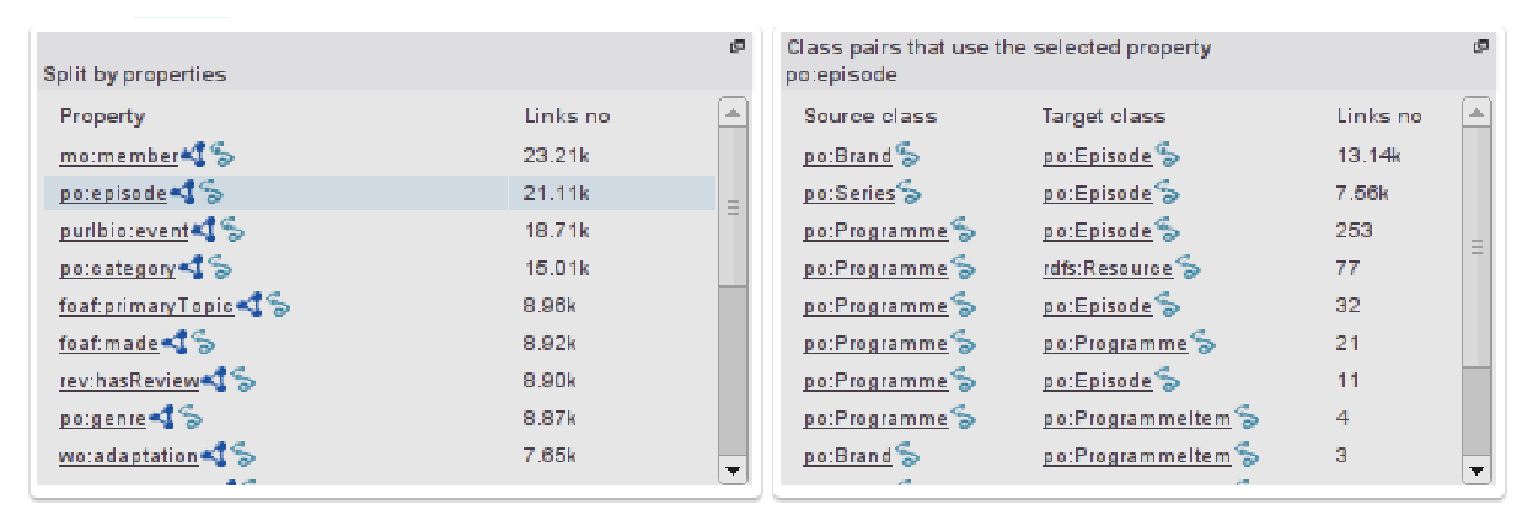
\includegraphics[scale=1]{images/applications/split-properties.eps}
            }
        \end{figure}
        \begin{figure}
            \centering
            \resizebox{\textwidth}{!}{
                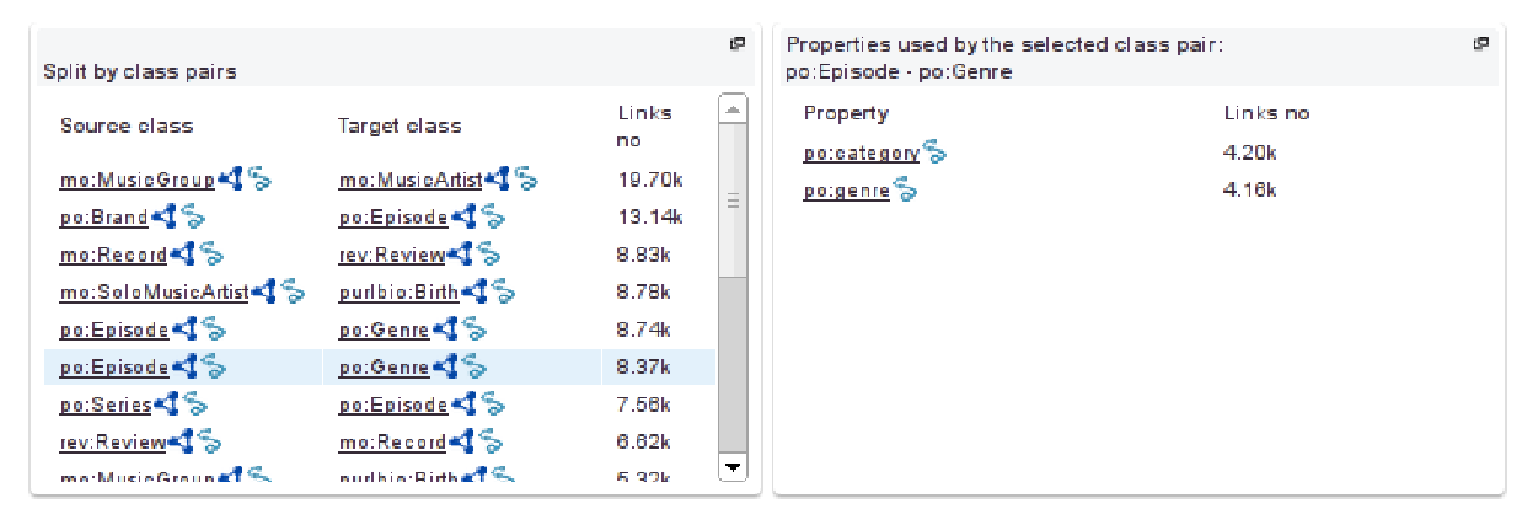
\includegraphics[scale=1]{images/applications/split-classes.eps}
            }
        \end{figure}
    \end{columns}
    \setbeamercovered{invisible}
    \begin{tikzpicture}[remember picture]
        %\draw[step=1cm,gray,ultra thick,overlay] (0,0) grid (12,12);

        \uncover<2-2>{
            \draw[red,ultra thick,overlay] (-.4,3.1) rectangle (3.5,5.5);
        }
        \uncover<3-3>{
            \draw[red,ultra thick,overlay] (-.4,2.4) rectangle (3.5,-.1);
        }
        \uncover<4-4>{
            \draw[red,ultra thick,overlay] (4.1,3.1) rectangle (11.2,5.5);
            \draw[red,thick,overlay] (5,4.65) edge[->,>=stealth'] (7.8,4.65);
        }
        \uncover<5-5>{
            \draw[red,ultra thick,overlay] (4.1,2.4) rectangle (11.2,-.1);
            \draw[red,thick,overlay] (5.3,.65) edge[->,>=stealth'] (7.8,1.65);
        }
    \end{tikzpicture}
    \setbeamercovered{transparent}
}

%\frame{
    %\frametitle{Inside the Dataset View}
    %\begin{figure}
        %\centering
        %\resizebox{!}{.8\textheight}{
            %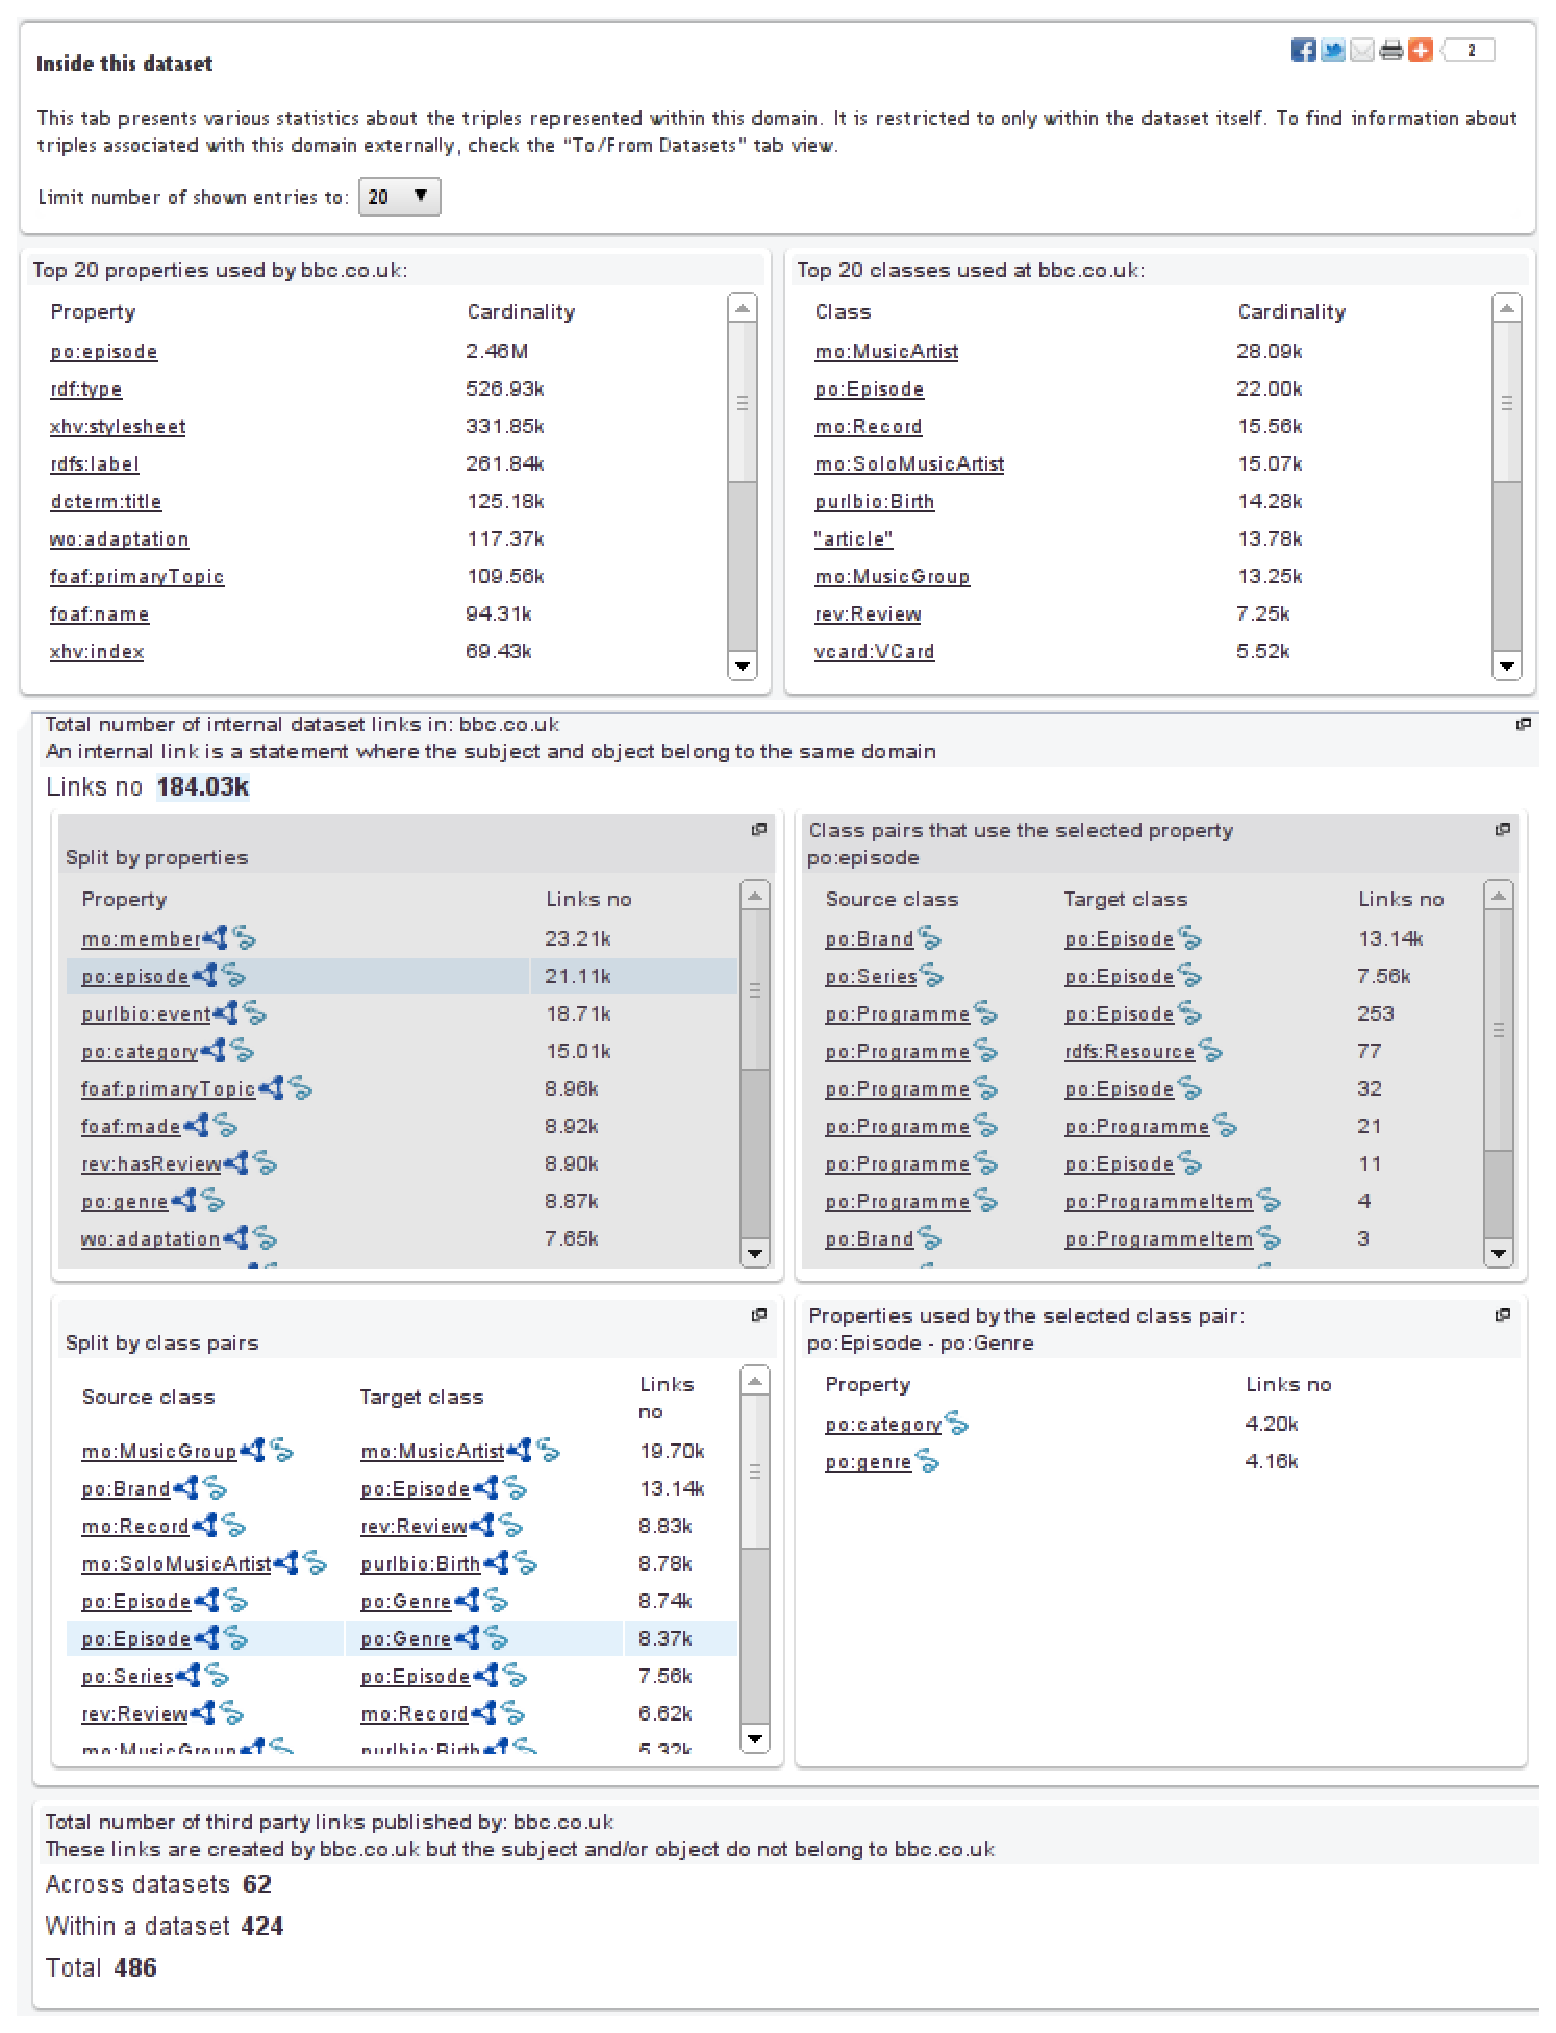
\includegraphics[scale=1]{images/applications/insideThisDataset.eps}
        %}
    %\end{figure}
%}

\frame{
    \frametitle{To/From the Dataset View}
    \vspace{.6cm}
    \begin{figure}
        \centering
        \resizebox{.6\textwidth}{!}{
            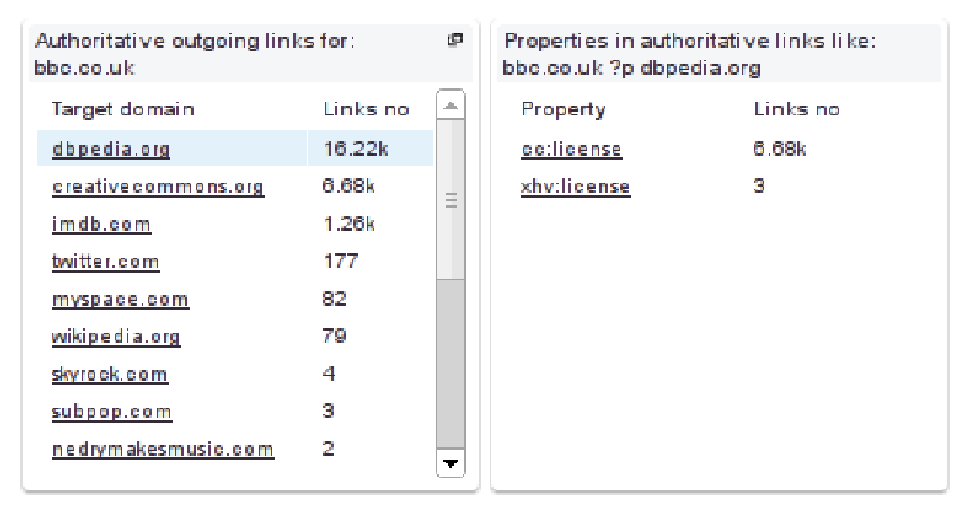
\includegraphics[scale=1]{images/applications/out-links.eps}
        }
    \end{figure}
    \vspace{-.3cm}
    \begin{figure}
        \centering
        \resizebox{.6\textwidth}{!}{
            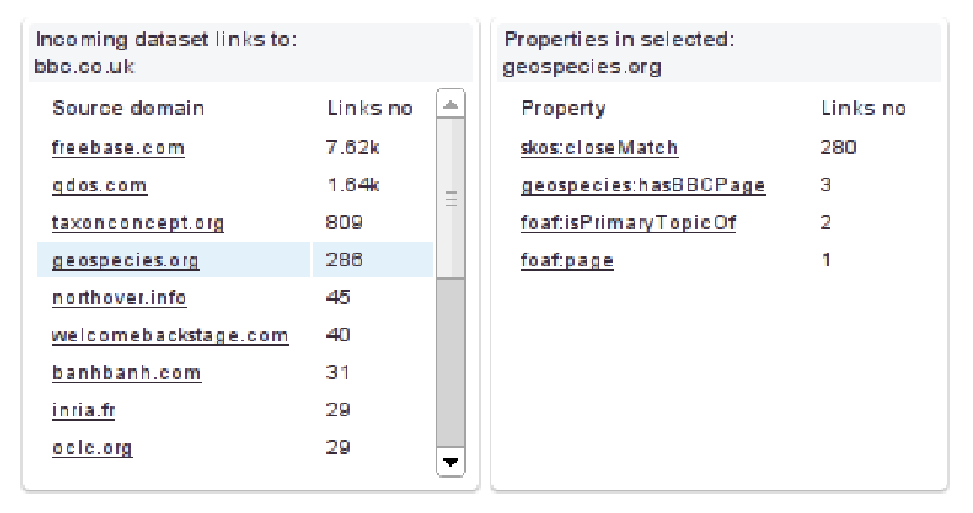
\includegraphics[scale=1]{images/applications/in-links.eps}
        }
    \end{figure}
    \setbeamercovered{invisible}
    \begin{tikzpicture}[remember picture]
        %\draw[step=1cm,gray,ultra thick,overlay] (0,0) grid (12,12);

        \uncover<2-2>{
            \draw[red,ultra thick,overlay] (2.1,4.1) rectangle (8.7,7.5);
            \draw[red,thick,overlay] (3.3,6.5) edge[->,>=stealth'] (5.5,6.5);
        }
        \uncover<3-3>{
            \draw[red,ultra thick,overlay] (2.1,.6) rectangle (8.7,4.1);
            \draw[red,thick,overlay] (3.65,2.3) edge[->,>=stealth'] (5.5,3);
        }
    \end{tikzpicture}
    \setbeamercovered{transparent}
}

%\frame{
    %\frametitle{To/From the Dataset View}
    %\begin{figure}
        %\centering
        %\resizebox{!}{.8\textheight}{
            %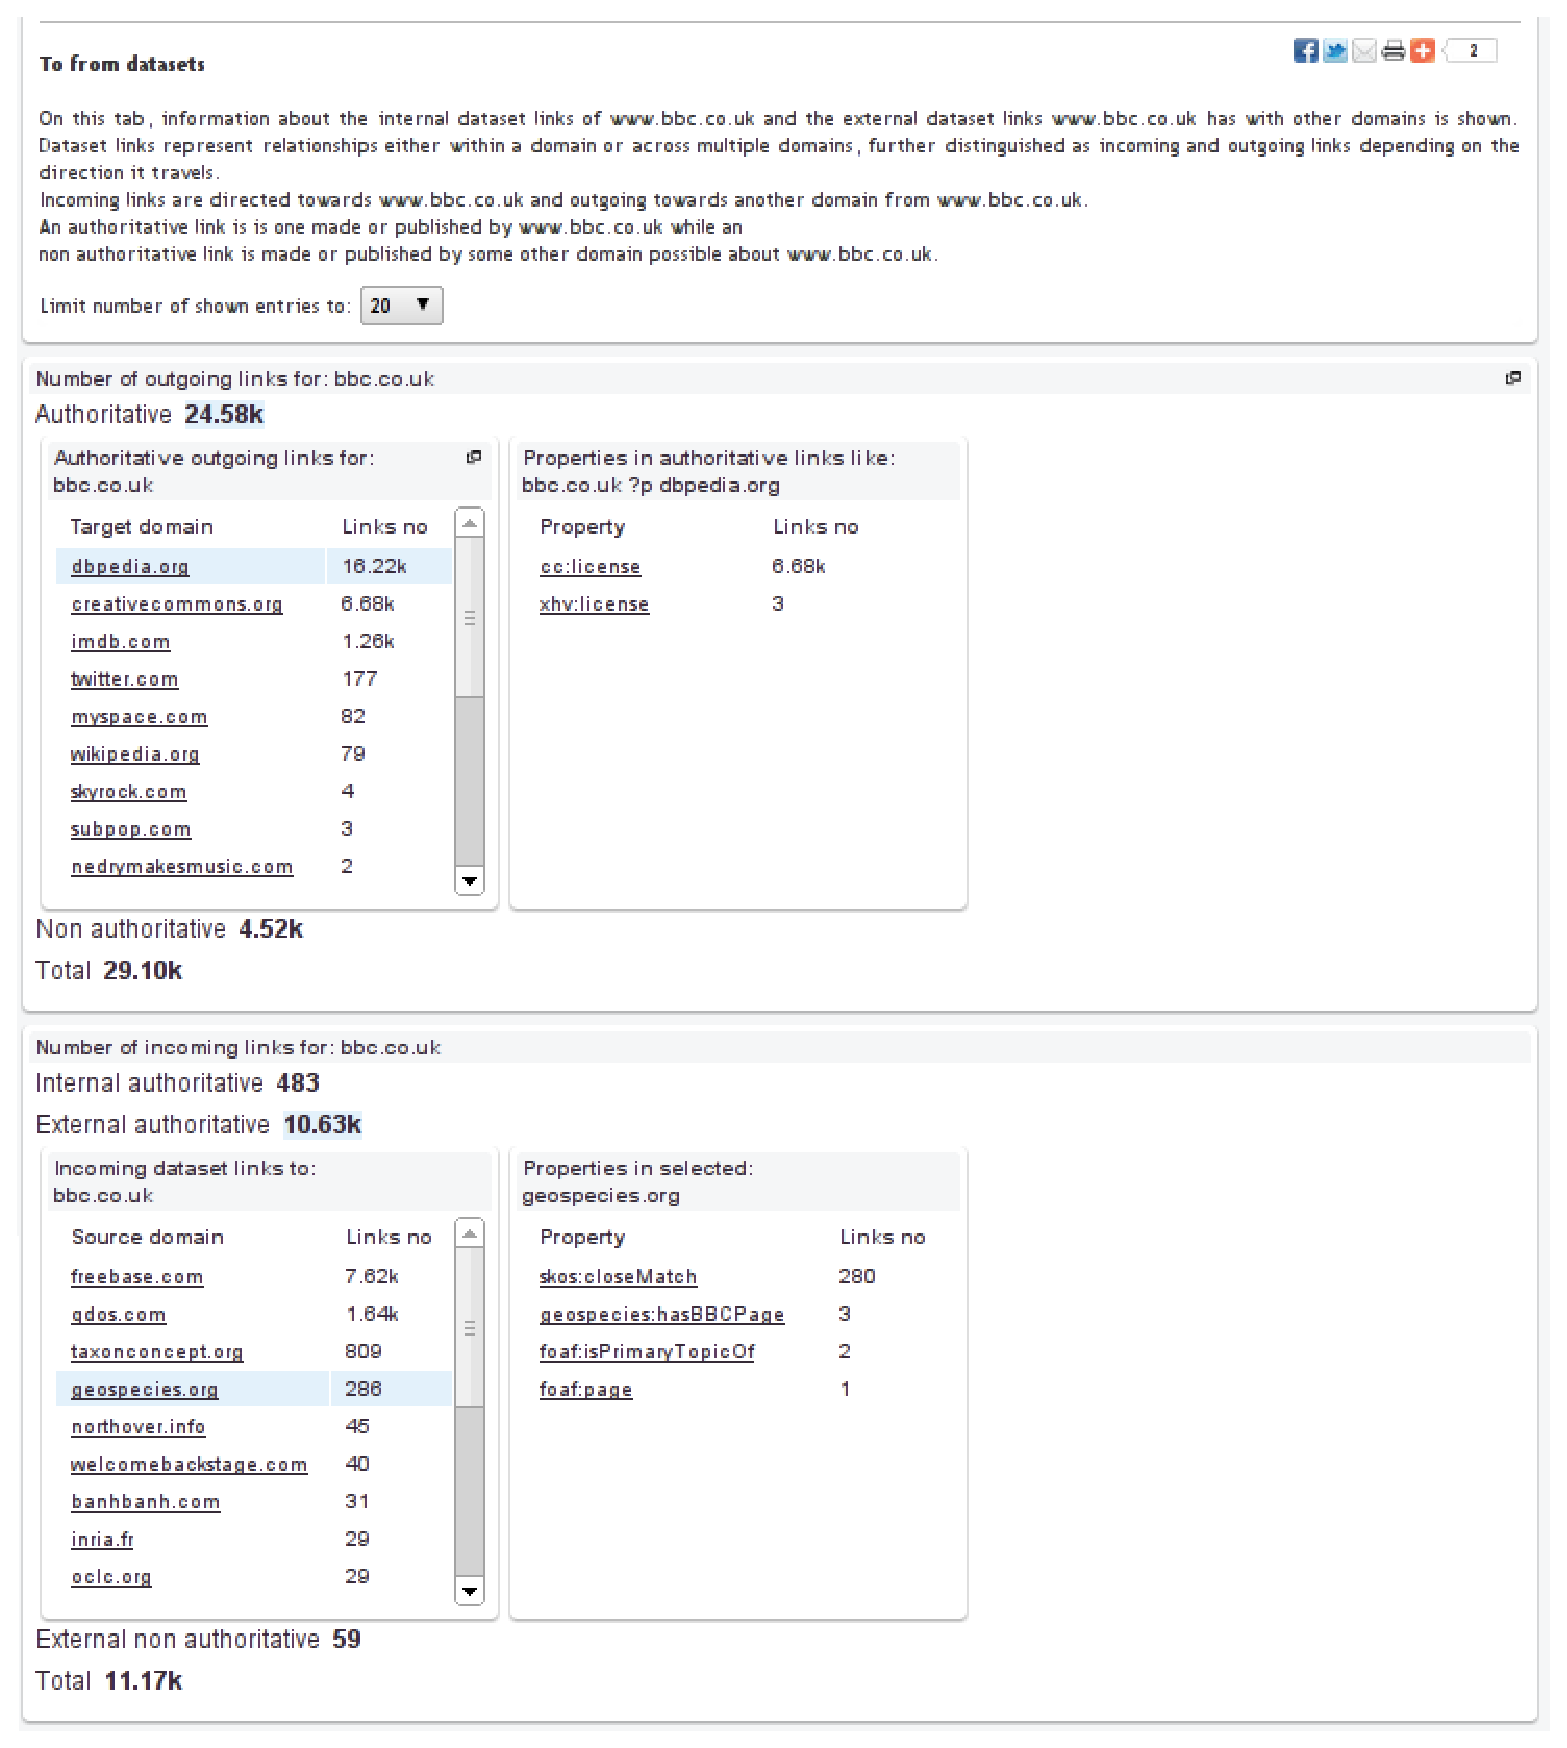
\includegraphics[scale=1]{images/applications/toFromDataset.eps}
        %}
    %\end{figure}
%}

\frame{
    \frametitle{Third-party Links View}
    \begin{figure}
        \centering
        \resizebox{.7\textwidth}{!}{
            
\includegraphics[scale=1]{images/applications/third-party.eps}
        }
    \end{figure}
    \setbeamercovered{invisible}
    \begin{tikzpicture}[remember picture]
        %\draw[step=1cm,gray,ultra thick,overlay] (0,0) grid (12,12);

        \uncover<2-2>{
            \draw[red,thick,overlay] (3.2,2.5) edge[->,>=stealth'] (5.5,3.8);
        }
    \end{tikzpicture}
    \setbeamercovered{transparent}
}

%% vim: et:sw=4


\section{Conclusion}

\frame{
    \frametitle{Summary And Directions for Future Research}
    \begin{columns}[c]
        \column{.3\textwidth}
        \begin{figure}
            \resizebox{.9\textwidth}{!}{
                \begin{tikzpicture}
                    \begin{axis}[
                            ybar,
                            symbolic x coords={Nodes,Edges},
                            enlargelimits=0.25, 
                            x=2cm,
                            bar width=0.3cm,
                            xtick=data,
                            ymajorgrids = true,
                            legend style={at={(0.5,-0.15)},
                            anchor=north,legend columns=1},
                        ]
                        \addplot coordinates {
                                (Nodes, 65042837)
                                (Edges, 233051608)
                            };

                        \addplot coordinates {
                                (Nodes, 1450687)
                                (Edges, 19725084)
                            };
                        \legend{DBpedia 2013 (en),Types Summary}
                    \end{axis}
                    %\draw[step=1cm,gray,ultra thick] (0,0) grid (3,5);
                    \draw[red,ultra thick] (.4,2.2) edge[->,>=stealth'] node[above right] {\textbf{$96\%$}} (.7,1.1);
                    \draw[red,ultra thick] (2.4,4.8) edge[->,>=stealth'] node[above right] {\textbf{$92\%$}} (2.7,1.4);
                \end{tikzpicture}
            }
        \end{figure}
        \column{.7\textwidth}
        \begin{description}
            \item<2->[Summary Updates:] Efficiently updates the summary of a dataset without avoiding to re-do the process from scratch.
            \item<3->[Data Quality:] Improve the data modeling by identifying structural inconsistencies.
            \item<4->[Approximate Summaries:] Develop summarisation relations which have little impact on the connectivity precision, and yet generate small summaries.
        \end{description}
    \end{columns}
}


\frame{
    \frametitle{Graph Ranking}
    \resizebox{\textwidth}{!}{
        \begin{figure}
            \centering
            \begin{subfigure}{.2\textwidth}
                \centering
                \resizebox{\textwidth}{!}{
                    \begin{tikzpicture}[->,>=stealth',every node/.style={draw,circle},node distance=2cm]
\node (0) {$v_0$};
\node[below left of = 0] (1) {$v_1$};
\node[below of = 0] (2) {$v_2$};
\node[below right of = 0] (3) {$v_3$};
\node[below of = 3] (4) {$v_4$};
\node[below of = 2] (5) {$v_5$};

\path[every node/.style={font=\footnotesize,fill=white}]
(0) edge node {a} (1)
 edge node {b} (2)
 edge node {c} (3)
(3) edge node {d} (4)
(2) edge node {d} (5)
 edge node {d} (4)
;
\end{tikzpicture}
                }
            \end{subfigure}
            \quad
            \begin{subfigure}{.2\textwidth}
                \centering
                \resizebox{\textwidth}{!}{
                    \usetikzlibrary{positioning}

\begin{tikzpicture}[every node/.style={draw,circle},node distance=.8cm]

\node (0) {$v_0$};
\node[dashed,below left = of 0 ] (a) {a};
\node[dashed,below = of 0 ] (b) {b};
\node[dashed,below right = of 0 ] (c) {c};

\node[below = of a ] (1) {$v_1$};
\node[below = of b ] (2) {$v_2$};
\node[below = of c ] (3) {$v_3$};

\node[dashed,below = of 2 ] (d2) {d};
\node[dashed,below = of 3 ] (d3) {d};

\node[below = of d3 ] (4) {$v_4$};
\node[below = of d2 ] (5) {$v_5$};

\path[->,every node/.style={font=\footnotesize,fill=white}]
(0) edge (a)
	edge (b)
	edge (c)
(a) edge (1)
(b) edge (2)
(c) edge (3)
(2) edge (d2)
(3) edge (d3)
(d2) edge (4) edge (5)
(d3) edge (4)
;

\end{tikzpicture}
                }
            \end{subfigure}
            \quad
            \begin{subfigure}{.6\textwidth}
                \centering
                \resizebox{\textwidth}{!}{
                    \begin{tikzpicture}[->,>=stealth',circ/.style={draw,circle},node distance=.8cm]
    \node (agg0) {$*$};

    \path (agg0) ++(-150:3) node[circ] (0) {$v_0$};

    \path (agg0) ++(-120:3) node (agg1) {$*$} ++(-110:2) node[dashed,circ] (a) {a};
    \path (agg1) ++(-70:2) node[circ] (1) {$v_1$};

    \path (agg0) ++(-60:3) node (agg2) {$*$} ++(-130:1.5) node[dashed,circ] (b) {b};
    \path (agg2) ++(-50:1.5) node[circ] (2) {$v_2$};
    \path (agg2) ++(-90:2) node (agg4) {$*$};

    \path (agg4) ++(-130:2) node[dashed,circ] (d2) {d};
    \path (agg4) ++(-90:2) node[circ] (5) {$v_5$};
    \path (agg4) ++(-40:2.3) node[circ] (4) {$v_4$};

    \node[right = 3cm of agg2] (agg3) {$*$};
    \path (agg3) ++(-130:1.5) node[dashed,circ] (c) {c};
    \path (agg3) ++(-50:1.5) node[circ] (3) {$v_3$};
    \path (agg3) ++(-90:2) node (agg5) {$*$} ++(-90:1.5) node[dashed,circ] (d3) {d};

    \path
        (agg0) edge (0) edge (agg1) edge (agg2) edge (agg3)
        (agg1) edge (a) edge (1)
        (agg2) edge (b) edge (2) edge (agg4)
        (agg3) edge (c) edge (3) edge (agg5)
        (agg4) edge (d2) edge (4) edge (5)
        (agg5) edge (d3) edge (4);
\end{tikzpicture}
%% vim: et:sw=4

                }
            \end{subfigure}
        \end{figure}
    }
}

\end{document}
%% vim: et:sw=4
